\documentclass[conference]{IEEEtran}
\IEEEoverridecommandlockouts
% The preceding line is only needed to identify funding in the first footnote. If that is unneeded, please comment it out.
\usepackage{cite}
\usepackage{amsmath,amssymb,amsfonts}
\usepackage{algorithmic}
\usepackage{graphicx}
\usepackage{textcomp}
\usepackage{booktabs}
\usepackage[table,xcdraw]{xcolor}
\usepackage{longtable}
\usepackage{multicol} % Pembuatan kolom ganda
\usepackage{multirow} % Pembuatan baris ganda
\usepackage{xcolor}
\def\BibTeX{{\rm B\kern-.05em{\sc i\kern-.025em b}\kern-.08em
    T\kern-.1667em\lower.7ex\hbox{E}\kern-.125emX}}
\begin{document}

\title{Reconstruction of Buried Irregular Objects on Concrete Based on Ground-Penetrating Radar Signals Using Generative Adversarial Network\\}

\author{\IEEEauthorblockN{1\textsuperscript{st} John Parulian Siahaan}
\IEEEauthorblockA{\textit{Department of Computer Engineering} \\
\textit{Faculty of Intelligent Electrical and Informatics Technology}\\
\textit{Sepuluh Nopember Institute of Technology}\\
Surabaya, Indonesia \\
07211940000040@mhs.its.ac.id}
\and
\IEEEauthorblockN{2\textsuperscript{nd} Dion Hayu Fandiantoro, S.T.,M.T.}
\IEEEauthorblockA{\textit{Department of Computer Engineering} \\
\textit{Faculty of Intelligent Electrical and Informatics Technology}\\
\textit{Sepuluh Nopember Institute of Technology}\\
Surabaya, Indonesia \\
dion@its.ac.id}
\and
\IEEEauthorblockN{3\textsuperscript{rd} Arief Kurniawan, S.T., M.T.}
\IEEEauthorblockA{\textit{Department of Computer Engineering} \\
\textit{Faculty of Intelligent Electrical and Informatics Technology}\\
\textit{Sepuluh Nopember Institute of Technology}\\
Surabaya, Indonesia \\
arifku@ee.its.ac.id}
}

\maketitle

\begin{abstract}
  Ground Penetrating Radar (GPR) has often been used in geophysics to detect objects buried underground. 
  Not only in soil media, other media such as wood, concrete and road can also be used. 
  The detected object can also be in various shapes and materials, one of which is the cavities. 
  Cavities are some air-space that arise in concrete due to air trapped in the casting process. 
  By using the GPR signal, efforts to detect these cavities can be carried out. 
  In this research, the signal reconstruction process from the GPR B-Scan was carried out. 
  The signal form that will be used is the ricker wavelet, because the shape is very good at forming seismic data. 
  The signal completion process generally uses the Fourier transform when integrating A-Scan signals, so it is relatively complicated and long. 
  By applying the conditional generatif adversial network (CGAN), GPR B-Scan data can be synthesized using the Generator and Discriminator functions. 
  These data can be used in identifying and classifying objects in the GPR signal, which is the focus of this research in the form of irregular shape cavities in concrete. 
  With this research, it is expected to form a method that can reconstruct the GPR B-Scan signal to make it simpler, which can then detect irregular shape cavities in concrete.
\end{abstract}

\begin{IEEEkeywords}
  Irregular, GPR, B-Scan, CGAN.
\end{IEEEkeywords}

\section{Introduction}
Ground penetrating radar (GPR) is a noninvasive geophysical method for detecting shallow subsurface electrical discontinuities. 
GPR works by sending electromagnetic (EM) pulses below the surface and the reflected waves are recorded by an antenna on the surface. 
Researchers often use GPR to study shallow subsurface strata and to identify anomalous underground structures in many near-surface applications \cite{a1}. 
Cavity is an object that can be identified using GPR.

Cavity in concrete is an empty cavity that forms inside or on the surface of the concrete. 
The shape of the cavity in ordinary concrete is irregular because the small cavities are joined together into one. 
According to BPSDM PUPR, damage to concrete due to air voids is included in damage code 201 \cite{a2}. 
This type of damage usually occurs due to a less dense mixing process, causing the concrete to lose its resistance. 
Therefore, GPR can be used to identify the size and position of voids beneath the concrete surface.

To obtain data on the shape of the subsurface geometric structure, the GPR raw data needs to be processed first. 
There are many solutions that have been made to process GPR data, both numerical methods such as Finite-Difference Time-Domain (FDTD) \cite{a3}, Method of Moments (MoM) \cite{a4}, and Finite Element Time-Domain (FETD) \cite{a5}, 
as well as GPR inversion methods such as ray-based tomography approaches \cite{a6}, reverse-time migration (RTM), \cite{a7}, and full-waveform inversion (FWI) \cite{a8}. 
However, this method is very complex in its interpretation. 
The interpretation of GPR data, both numerical methods and GPR inversions, is relatively complicated due to variations in the response of electromagnetic waves generated by various subsurface structures and materials. 
Deep geological knowledge or experience in data interpretation is required to avoid errors or find faults.

In recent years, there have been popular data-driven methods such as neural networks in applications in many scientific fields, with notable success especially in the fields of computer vision and natural language processing. 
Deep neural networks (DNNs) have demonstrated outstanding capabilities in applications related to image classification \cite{a9}, object detection \cite{a10}, semantic segmentation (pixel level prediction) \cite{a11} and image synthesis \cite{a12}. 
DNN automatically learns high-level features through training data and can then update nonlinear solutions between the input image data and various domain data, such as labels, text, or other images. 
Therefore, several inversion methods based on end-to-end deep learning have been proposed to freeze the velocity or impedance of the seismic data \cite{a13}.

A generative model is a part of a neural network that enables realistic data synthesis. 
Generative Adversarial Networks (GANs) is a form of generative model that has a generator function to generate new data through training (train) and a discriminator to determine whether the new data is fake or original data. 
Pix2pix is a GAN model that has the ability to translate image-to-image. 
This model has been successfully applied in various applications such as medical image processing, road demolition, interior design, and digital art. 
Therefore, this title is proposed with the hope that this GAN model can reconstruct irregular objects buried in concrete based on GPR signals.

Based on this background, the problem that can be taken is that the process of modeling cavities in concrete based on GPR signals is relatively complicated and long. 
There are many solutions that have been done to model subsurface objects, but these methods require complex calculation processes and long computational times. 
Therefore, a method is needed to quickly reconstruct buried irregular objects in concrete based on GPR signals.

The purpose of this study is to apply a generative model to reconstruct irregular objects buried in concrete based on GPR signals more quickly. 
With the implementation of this research, it is hoped that generative models can be applied to reconstruct irregularly buried objects in concrete based on high-resolution GPR signals in concrete using GANs. 
In addition, this study can also be a reference for further research related to GPR signal reconstruction.

\section{Related Research}
In carrying out this research, references are needed that can be used to assist research. 
Related research references include research \cite{b1}-\cite{b3}.

Research \cite{b1} is a study related to the application of the GAN method to detect subsurface objects. 
In his research, the objects detected were cylinders with 3 types of materials, namely iron, plastic, and concrete buried beneath the surface of the soil. 
This research also still uses the FDTD method in its model. 
The results of this study indicate that the GAN method can be used on GPR data, both from original data and GPR simulation data. 
Class conditioning can be applied to the GAN method in producing labeled training data for the classifier.

Research \cite{b2} is a study that uses 2 methods to detect cavities in freshly printed concrete, namely the Infrared Thermographic and GPR approaches. 
Research with the GPR approach aims to determine the limitations of using GPR in post-cast concrete. 
To avoid damage to the concrete after casting, a plywood board is used as a GPR cross section so that it does not touch the concrete directly. 
The results showed that GPR could be a non-destructive testing (NDT) method to detect cavities with a size of 3.8 cm to 10 cm, 3 hours after placing the concrete.

Research \cite{b3} is research related to the use of Conditional Adversial Networks (CGAN) in changing from one image to another. 
This study demonstrates the use of pix2pix in synthesizing photos from rough labels to an image of a particular object. 
Philip Isola and his team concluded that the use of CGAN is very promising in the problem of changing one image to another, especially those that require structured output.

Based on the reference research, a research was conducted entitled "Reconstruction of Buried Irregular Objects on Concrete Based on Ground-Penetrating Radar Signals Using Generative Adversarial Network". 
This research takes the idea from \cite{b1} to use the GAN method to detect subsurface buried objects. 
This research also takes the idea from \cite{b2} in detecting cavities in the subsurface of concrete using GPR. 
This study also uses \cite{b3}'s method to change from B-scan images to predictive images of the shape and position of objects below the concrete surface.

\section{Methodology}
This research was carried out according to the methodology that had been designed. 
The methodology is divided into 4 stages, namely GPR datasets, GANs architecture, training model, and model evaluation. 
Figure \ref{fig:metodologi} shows a diagram of the research methodology

\begin{figure}[ht]
  \centering
  
\includegraphics[scale=0.35]{gambar/metodologiEN.png}
  \caption{Diagram of the Research Methodology}
  \label{fig:metodologi}
\end{figure}

\subsection{GPR Datasets}\label{DatasetGPR}
This stage is the stage of collecting the GPR dataset. 
There are 2 types of data needed, namely input data in the form of GPR B-scan images from gprMax simulation results and expected output data in the form of geometric shapes from GPR B-scan images. 
The flow of the dataset collection process is shown in Figure \ref{fig:datasetgpr}.

\begin{figure}[ht]
  \centering
  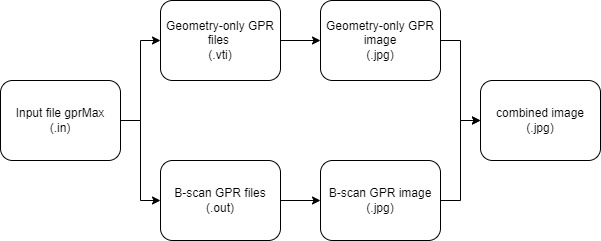
\includegraphics[scale=0.35]{gambar/alur pengumpulan data EN.png}
  \caption{Diagram of GPR Dataset Collection}
  \label{fig:datasetgpr}
\end{figure}

The simulation uses gprMax to produce output files of simulated geometric shapes and GPR B-scan output files using gprMax input files. 
Every need and how to install gprMax can be found on the gprMax github. 
In installing gprMax, it is required to install Python, Miniconda/Anaconda, and a C Compiler which supports OpenMP (Desktop development with C++ on Visual Studio for Windows OS). \\

In compiling the GPR input program code, it takes several building parameters that need to be considered. 
The constituent parameters can be seen in the gprMax guide on the official gprMax website. 
In this study, the system parameters created in the GPR dataset can be seen in table \ref{tb:inputGPR}. 
An example of using parameters in the input file can also be seen in figure \ref{fig:inputgprMax}.

\begin{table}[htbp]
    \caption{GprMax Input Parameters}
    \begin{center}
    \begin{tabular}{|c|c|c|}
    \hline
    \textbf{Parameter} & \textbf{Value} \\
    \hline
    Dimensions                    & 0.3 m x 0.3 m x 0.001 m                   \\
    Time Windows                  & 3 ns                                      \\
    Material                      & Concrete (medium) and free space (object) \\
    Signal Base                   & Ricker                                    \\
    Source Flow Direction         & 0.001 m/step to the X-axis                \\
    Object Shape                  & cylinder                                  \\
    \hline
    \end{tabular}
    \label{tb:inputGPR}
    \end{center}
\end{table}

\begin{figure}[ht]
  \centering
  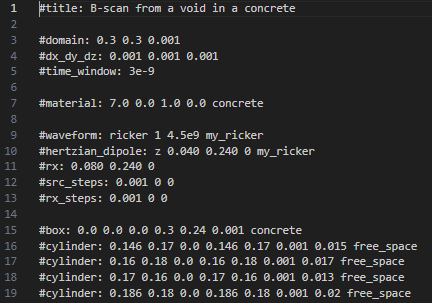
\includegraphics[scale=0.6]{gambar/inputGprMax.png}
  \caption{Example of the GprMax Input File}
  \label{fig:inputgprMax}
\end{figure}

The gprMax input data above is then simulated with 2 different tools to produce an output file of simulated geometric shapes and a GPR B-scan output file. 
From the simulation process, two results are obtained, namely the output file of the simulation geometry shape (.vti) and the output file of B-scan GPR (.out). 
To obtain an image of a simulated geometric shape, the output file of the simulated geometric shape is run using the Paraview application. 
Meanwhile, to obtain an image of the shape of the GPR B-scan signal, the output file of the GPR B-scan is run using tools from gprMax.

These two types of images are then combined into one image using the PIL library. 
The two images will be arranged horizontally, where the left image is a gprMax B-scan image and the right image is a geometric shape image. 
An example of a combined image is shown in Figure \ref{fig:contohdata}. 
This combined image then becomes the GAN model dataset that will be formed, which in this study uses a total of 200 data.

\begin{figure}[ht]
  \centering
  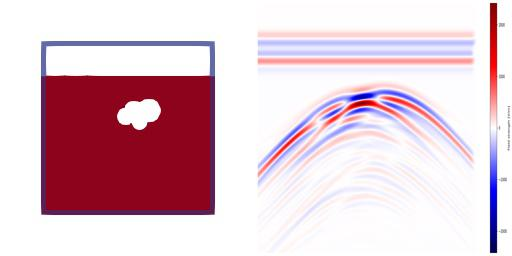
\includegraphics[scale=0.5]{gambar/data1.jpg}
  \caption{Combined image of the subsurface geometry (left) with the simulated GPR B-scan shape (right)}
  \label{fig:contohdata}
\end{figure}

\subsection{GANs Architecture}
After the dataset has been successfully collected, a GAN model will then be formed. 
The GAN model to be formed uses the Pix2pix Conditional GAN model. 
The GAN architecture will be divided into 2 parts, namely the generator part which functions to synthesize images like the original data, and the discriminator part which functions to distinguish between the original data and the synthesized data. 
The diagram of the GAN architecture is shown in Figure \ref{fig:arsitekturGAN}.

\begin{figure}[ht]
  \centering
  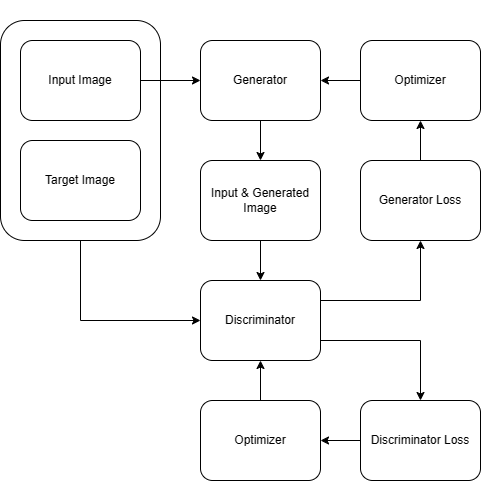
\includegraphics[scale=0.45]{gambar/Arsitektur GAN.png}
  \caption{Diagram of Formed GAN Architecture}
  \label{fig:arsitekturGAN}
\end{figure}

In the generator section, the U-net architecture is used \cite{c1}. 
This architecture consists of an encoder network followed by a decoder network. 
Encoder network will apply Convolution process $>>$ Batch normalization $>>$ Leaky ReLU. 
While the decoder will apply the Transposed convolution process $>>$ Batch normalization $>>$ Dropout (for the first 3 blocks) $>>$ ReLU. 
Each encoder-decoder pair has a skip connection that functions to capture any low-level information that is shared between input and output. 
Generator architecture diagram can be seen in the figure \ref{fig:generator}.

\begin{figure}[ht]
  \centering
  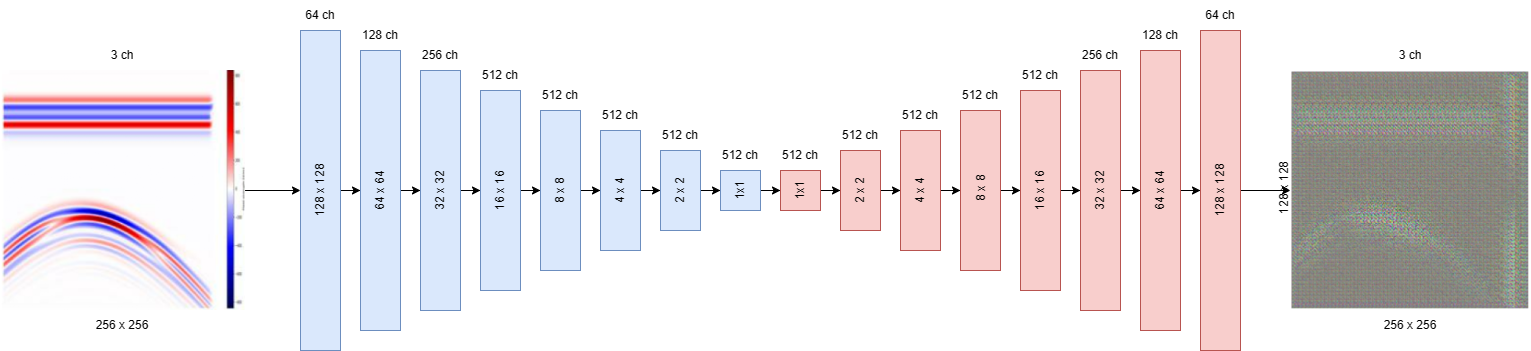
\includegraphics[scale=0.15]{gambar/Generator.png}
  \caption{Diagram of Generator Architecture}
  \label{fig:generator}
\end{figure}

In the discriminator section, the Convolutional Patch GAN architecture is used which will try to classify a patch (30 x 30) of the image as real or not. 
The discriminator will receive two pairs of images as input, namely the original-input image and the synthesis-input image. 
Each of these input pairs will be merged first before entering the encoder network.
The Discriminator architecture diagram can be seen in Figure \ref{fig:discriminator}.

\begin{figure}[ht]
  \centering
  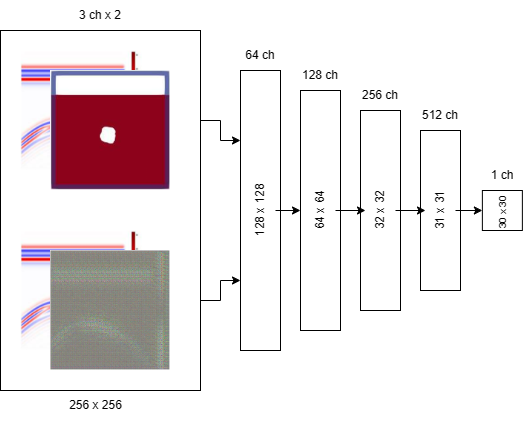
\includegraphics[scale=0.3]{gambar/Discriminator.png}
  \caption{Diagram of Discriminator Architecture}
  \label{fig:discriminator}
\end{figure}

Generator Loss is a combination of sigmoid cross-entropy loss between the resulting image with an array 1 (GAN Adversial Loss), and MAE (Mean Absolute Error) between the synthesized image and the original image (L1 Loss).
Mathematically, the value of Total Generator Loss can be defined as

\begin{equation}
  \label{eq:genLoss}
  Total Gen Loss = GAN Adversial Loss + (\lambda * L_{1} Loss) 
\end{equation}

where $\lambda$ can be defined as the model wants (in this study $\lambda$ = 100).

Discriminator Loss consists of sigmoid cross-entropy loss between the original image and array 1 (Real Loss), and sigmoid cross-entropy loss between the resulting image and array 0 (Generated Loss).
Total Discriminator Loss is the sum of Real Loss and Generated Loss.

The GAN model also defines optimizer and checkpoint functions.
The optimizer function uses Adaptive Moment Estimation (Adam) for both generator and discriminator.
The checkpoint function is used to store temporary results (checkpoints) from the training results of the GAN model generator and discriminator.

\subsection{Training Model}
The GAN architecture that has been formed is then forwarded to the training process.
The overall flow of the Training Model can be seen in Figure \ref{fig:arsitekturGAN}.
Of the 200 data in the dataset, 160 are used for the model training process.
The training process for this model was carried out in 40,000 iterations.
For every 1000 iterations, the image synthesis process is displayed, and for every 5000 iterations the checkpoints of the model are stored.

\begin{figure}[ht]
  \centering
  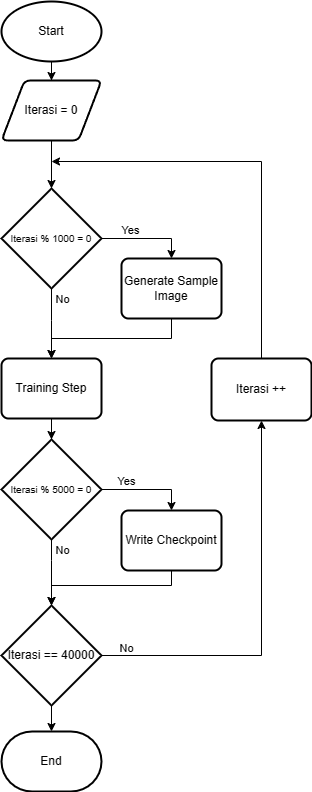
\includegraphics[scale=0.5]{gambar/Training_model.png}
  \caption{Diagram of Overall Model Training Process}
  \label{fig:training}
\end{figure}

For every 1 iteration of the training process, the model will run a process whose flow can be seen in Figure \ref{fig:training}.
The Input Image will be entered into the Generator, and will generate a synthesis Image.
The discriminator will process 2 input pairs, namely the input image pair with the original image, and the input image pair with the synthesized image.
In the first pair, the discriminator output from the original image will be obtained, and the second pair will obtain the discriminator output from the synthesized image.

The Loss Generator will process the Discriminator output from the synthesized image, together with the synthesized image and the original image.
The result of the Total Generator Loss will be received by the Generator Optimizer, and will be applied to the Generator in the next iteration.
Discriminator Loss will process Discriminator output from the synthesized image and from the original image.
The results of the Total Discriminator Loss will be received by the Discriminator Optimizer, and will be applied to the Discriminator in the next iteration.

\subsection{Evaluasi Model}
After the model has undergone a training process, the model will be tested using test data. 
The test data is in the form of 40 data from a dataset that has not been trained on the model. 
The last saved checkpoint will be loaded, and it will attempt to synthesize the image using the test data.

The evaluation process is carried out with a matrix evaluation followed by a visual evaluation. 
Matrix evaluation is an objective method that uses various metrics and numerical parameters to measure the degree to which two images match or differ. 
The matrix evaluation methods used in this study are the Root Mean Square (RMS), Mean Square Error (MSE) and Structural Similarity Index (SSIM) methods. 
RMS and MSE are generally used to measure the error or difference between two images or signals, with lower values indicating greater similarity. 
Whereas SSIM provides a more holistic measure of the structural similarity between two images.

After evaluating the matrix, a visual evaluation is carried out. 
Visual evaluation is carried out by involving subjective judgments by humans on the quality and similarity of two images. 
In assisting the visual evaluation process, the image differencing function is used. 
The image differencing function involves subtracting the pixels from the original image with the synthesized image. 
The subtraction results can reveal important information about structural changes, object shifts, or other changes in the image.

\section{Results and Discussion}

\subsection{GPR Datasets}
This study uses the GPR dataset from the gprMax simulation results. 
The gprMax simulation was carried out to obtain 2 types of data, namely GPR B-scan image data and simulated geometric shape image data. 
For B-scan image data it takes about 15-20 minutes per simulation, while for geometric shape image data it takes about 5-10 minutes per simulation. 
So that the total time needed to simulate 200 of the GPR B-scan image data and simulated geometric shape image data as well as merging the two data into one is around 85 hours.

Of the 200 GPR data, 160 data were used for the model training process and 40 data for the model evaluation process. 
The simulation parameters on this data are randomly generated with certain limits for the training data and are made to adjust the variations for the test data. 
The research dataset is varied based on the following categories.

\begin{enumerate}

  \item Regular-shaped object

  \item Complexity of the object

  \item Object size
  
  \item Position objects from the surface

\end{enumerate}

In the category of regular-shaped object variations, data is distinguished based on the regular shape of the object, namely data with circular objects (front view cylinders) and data with rectangular shaped objects (side view cylinders).
The object only consists of 1 constituent object, with a position and size that is freed, namely a position of about 2.5-10 cm below the surface and a size of about 3-10 cm.
An example of data for this variation can be seen in Figure \ref{fig:regularData}.

\begin{figure}[ht]
  \centering
  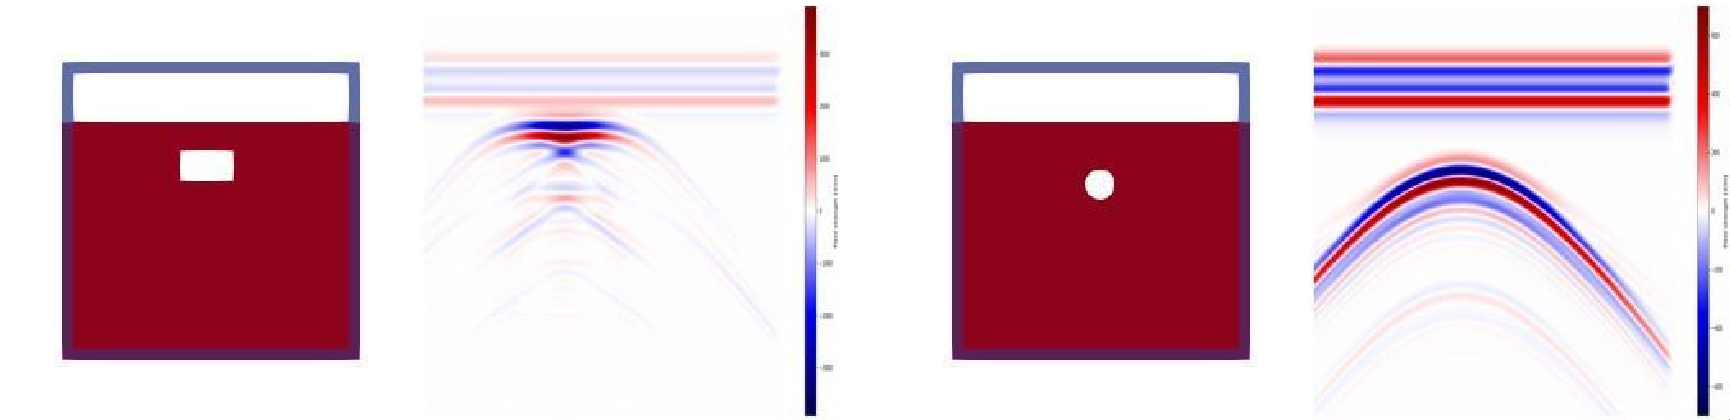
\includegraphics[scale=0.2]{gambar/variasi reguler.png}
  \caption{Data with Circle Shaped Objects (Right) and Data with Rectangular Objects (Left)}
  \label{fig:regularData}
\end{figure}

In the category of variations in the complexity of the shape of objects, data is distinguished based on the number of constituent objects that are combined, namely data with simple objects and data with complex objects.
Simple objects have around 3-6 constituent objects, while complex objects have around 10-15 constituent objects.
The position of the object and the size of the object making up the two data are equated, namely the position of about 6.5 cm below the surface and the size of the object making up about 1.5 cm.
An example of data for this variation can be seen in Figure \ref{fig:kompleksData}.

\begin{figure}[ht]
  \centering
  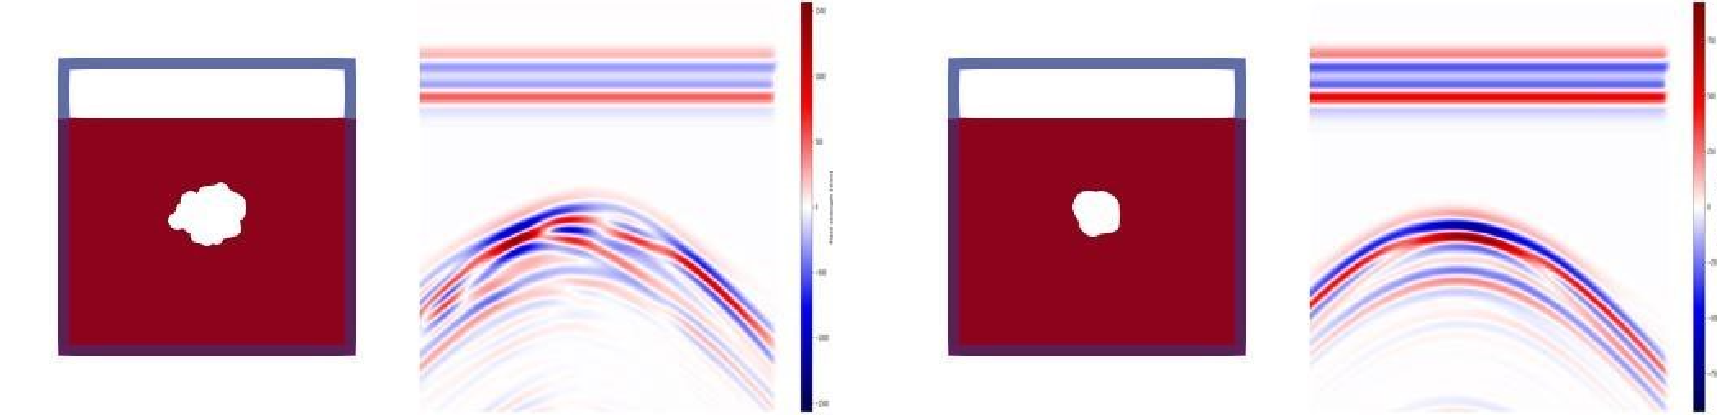
\includegraphics[scale=0.2]{gambar/variasi kompleksitas.png}
  \caption{Data with Simple Shaped Objects (Right) and Data with Complex Shaped Objects (Left)}
  \label{fig:kompleksData}
\end{figure}

In the object size variation category, data is distinguished based on the size of the object, namely data with small objects and data with large objects.
Small objects have a size of about 3-4 cm, while large objects have a size of about 5-6 cm.
The number of constituent objects and the position of the objects are equated, namely the constituent objects are a total of 5 pieces and a depth of about 4.5 cm.
An example of data for this variation can be seen in Figure \ref{fig:ukuranData}.

\begin{figure}[ht]
  \centering
  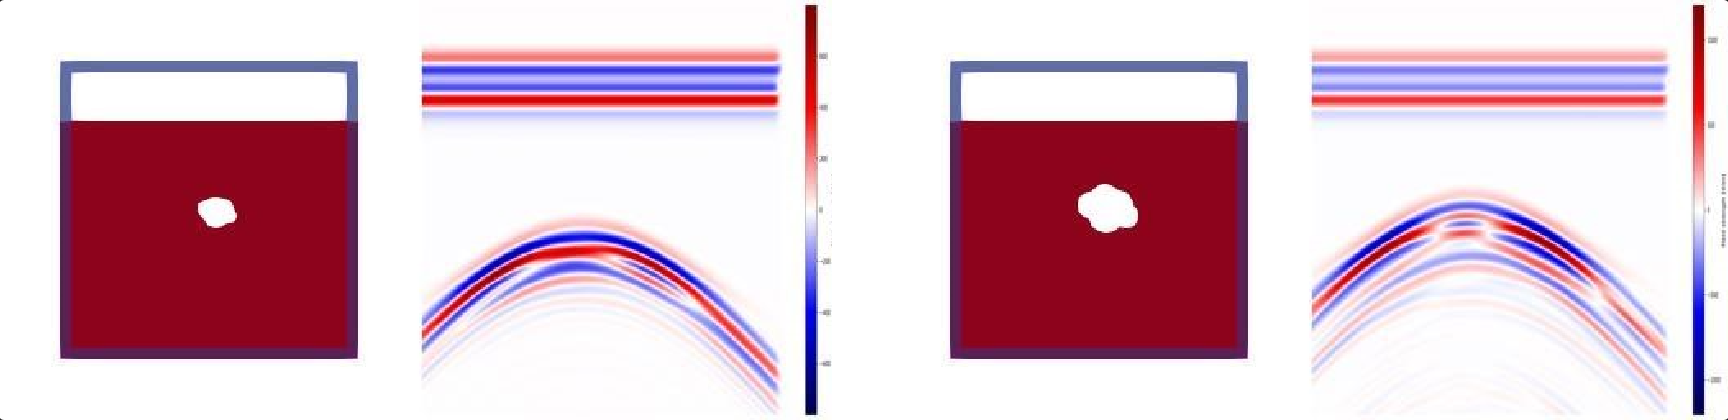
\includegraphics[scale=0.2]{gambar/variasi ukuran.png}
  \caption{Data with Large Objects (Right) and Data with Small Objects (Left)}
  \label{fig:ukuranData}
\end{figure}

In the category of variations in the position of objects below the surface, the data is differentiated based on the position of the object from the surface, namely data with shallow objects and data with deep objects.
Shallow objects have a position of about 2.5 cm from the surface, while deep objects have a position of about 7.5 cm from the surface.
The size of the object and the number of constituent objects are equated, namely the size of the object is around 4.5 cm and the number of constituent objects is 5 pieces.
An example of data for this variation can be seen in Figure \ref{fig:posisiData}.

\begin{figure}[ht]
  \centering
  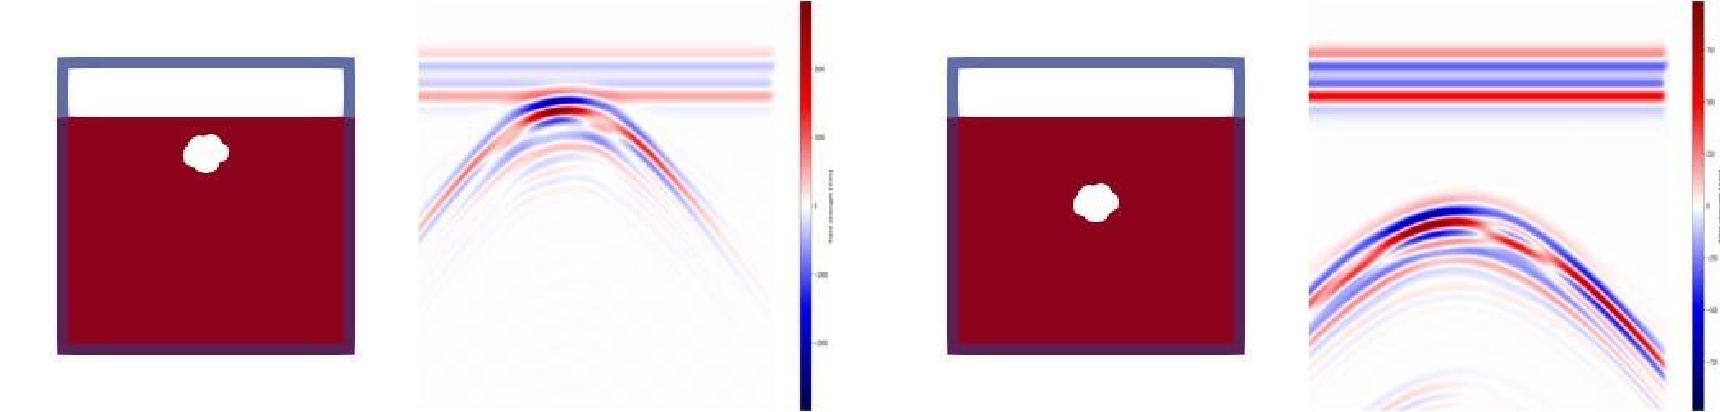
\includegraphics[scale=0.2]{gambar/variasi kedalaman.png}
  \caption{Data with the position of objects far from the surface (right) and data with the position of objects near the surface (left)}
  \label{fig:posisiData}
\end{figure}

\subsection{GAN Model Training Results}

The model training process was carried out in 40,000 iterations.
The total time required to carry out the entire training process for 9 hours from 20.00 WIB to 05.00 WIB the next day.
During training, the total discriminator loss and total generator loss values are stored in a log.
By using a tensorboard, the loss values stored in the log can be visualized in graphical form.

\begin{figure}[ht]
  \centering
  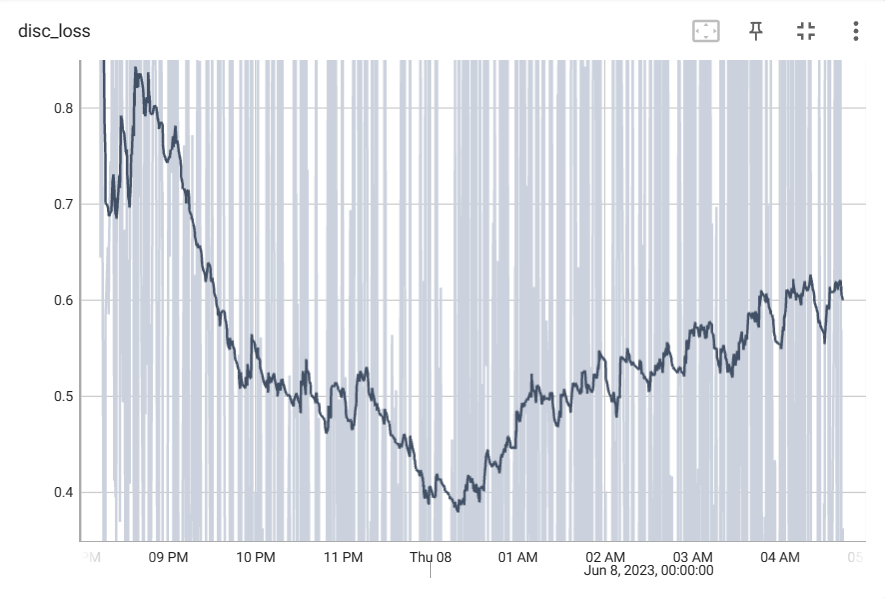
\includegraphics[scale=0.4]{gambar/Disc_loss.png}
  \caption{Total Discriminator Loss Graph}
  \label{fig:discLoss}
\end{figure}

Figure \ref{fig:discLoss} shows a graph of the discriminator loss which initially gets smaller then increases.
This shows that the initial discriminator is getting better at learning the differences between the original data and the synthesized data.
After passing a certain time, the discriminator then becomes increasingly difficult to study these differences.

\begin{figure}[ht]
  \centering
  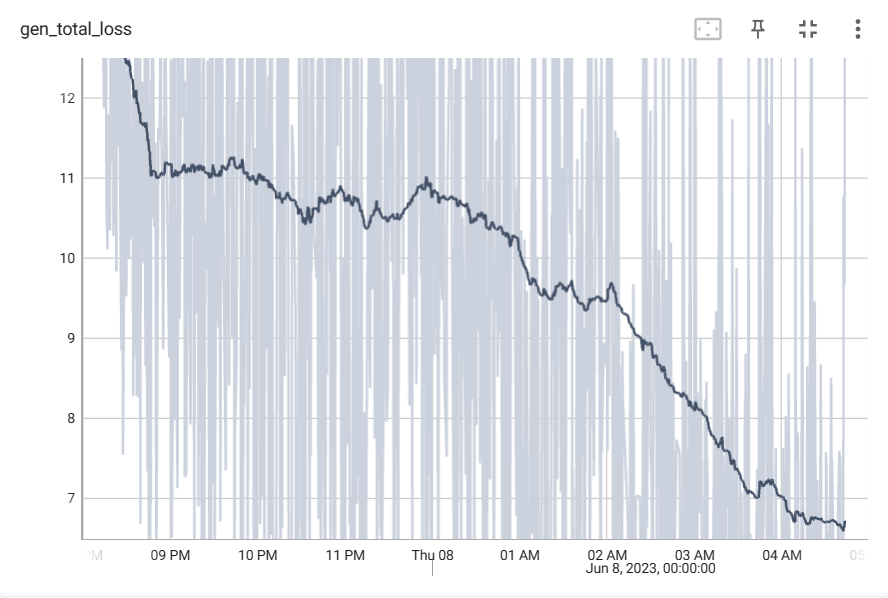
\includegraphics[scale=0.4]{gambar/Gen_total_loss.png}
  \caption{Total Generator Loss Graph}
  \label{fig:genLoss}
\end{figure}

Figure \ref{fig:genLoss} shows a graph of the generator loss which is getting smaller and smaller.
This shows that the generator is getting better at learning and producing synthesis data that matches the original data.
The graph also shows a fairly constant decrease in value, so it can be said that the generator model is well trained in the GAN model training process.

In the GAN model training process, it is important to compare the values or graphs of the loss generator and the discriminator loss.
In both graphs, it can be seen that initially the change in the two loss values decreases equally, which shows that the model process in studying the data is going well.
However, at around 00.00 the discriminator loss graph was increasing, while the loss generator graph was still decreasing.
This shows that at that time interval, the discriminator has difficulty differentiating the original image from the fake image, while the generator is still getting better at producing output that matches the original.

\subsection{GAN Output Evaluation Results}

The research data used 200 gprMax simulation data for GPR B-scan images along with the geometric shapes from the simulation.
Of the 200 total data, 40 data were used as test data and the GAN model was evaluated.
The evaluation process is carried out with a matrix evaluation followed by a visual evaluation.
Matrix evaluation was carried out using 3 methods, namely the RMS, MSE, and SSIM methods.
For the RMS and MSE results it is said to be good if the value is getting closer to 0, while for the SSIM result value it is said to be good if the value is getting closer to 1.
The results of the matrix evaluation for all data can be seen in table \ref{tb:evaluasimatriks}.

\begin{table}[]
  \caption{Table of RMS, MSE and SSIM Values from Synthesis Images with Original Images for Each Data Variation}
  \label{tb:evaluasimatriks}
  \begin{tabular}{|l|cc|cc|cc|}
  \hline
  \multicolumn{1}{|c|}{Data Variation}                  & \multicolumn{2}{c|}{RMS}                                                                               & \multicolumn{2}{c|}{MSE}                                                                                   & \multicolumn{2}{c|}{SSIM}                                                                            \\ \hline
                                                      & \multicolumn{1}{c|}{\cellcolor[HTML]{FFFFFF}0.256} & \cellcolor[HTML]{FFFFFF}                         & \multicolumn{1}{c|}{\cellcolor[HTML]{FFFFFF}0.072}  & \cellcolor[HTML]{FFFFFF}                           & \multicolumn{1}{c|}{\cellcolor[HTML]{FFFFFF}0.848} & \cellcolor[HTML]{FFFFFF}                        \\ \cline{2-2} \cline{4-4} \cline{6-6}
                                                      & \multicolumn{1}{c|}{\cellcolor[HTML]{FFFFFF}0.271} & \cellcolor[HTML]{FFFFFF}                         & \multicolumn{1}{c|}{\cellcolor[HTML]{FFFFFF}0.082}  & \cellcolor[HTML]{FFFFFF}                           & \multicolumn{1}{c|}{\cellcolor[HTML]{FFFFFF}0.811} & \cellcolor[HTML]{FFFFFF}                        \\ \cline{2-2} \cline{4-4} \cline{6-6}
                                                      & \multicolumn{1}{c|}{\cellcolor[HTML]{FFFFFF}0.265} & \cellcolor[HTML]{FFFFFF}                         & \multicolumn{1}{c|}{\cellcolor[HTML]{FFFFFF}0.078}  & \cellcolor[HTML]{FFFFFF}                           & \multicolumn{1}{c|}{\cellcolor[HTML]{FFFFFF}0.833} & \cellcolor[HTML]{FFFFFF}                        \\ \cline{2-2} \cline{4-4} \cline{6-6}
                                                      & \multicolumn{1}{c|}{\cellcolor[HTML]{FFFFFF}0.234} & \cellcolor[HTML]{FFFFFF}                         & \multicolumn{1}{c|}{\cellcolor[HTML]{FFFFFF}0.063}  & \cellcolor[HTML]{FFFFFF}                           & \multicolumn{1}{c|}{\cellcolor[HTML]{FFFFFF}0.837} & \cellcolor[HTML]{FFFFFF}                        \\ \cline{2-2} \cline{4-4} \cline{6-6}
  \multirow{-5}{*}{Simple Shapes}          & \multicolumn{1}{c|}{\cellcolor[HTML]{FFFFFF}0.249} & \multirow{-5}{*}{\cellcolor[HTML]{FFFFFF}0.255}  & \multicolumn{1}{c|}{\cellcolor[HTML]{FFFFFF}0.071}  & \multirow{-5}{*}{\cellcolor[HTML]{FFFFFF}0.073}       & \multicolumn{1}{c|}{\cellcolor[HTML]{FFFFFF}0.816} & \multirow{-5}{*}{\cellcolor[HTML]{FFFFFF}0.829} \\ \hline
                                                      & \multicolumn{1}{c|}{0.260}                         & \cellcolor[HTML]{FFFFFF}                         & \multicolumn{1}{c|}{0.075}                         & \cellcolor[HTML]{FFFFFF}                           & \multicolumn{1}{c|}{0.841}                         & \cellcolor[HTML]{FFFFFF}                        \\ \cline{2-2} \cline{4-4} \cline{6-6}
                                                      & \multicolumn{1}{l|}{0.246}                         & \cellcolor[HTML]{FFFFFF}                         & \multicolumn{1}{l|}{0.068}                         & \cellcolor[HTML]{FFFFFF}                           & \multicolumn{1}{l|}{0.830}                         & \cellcolor[HTML]{FFFFFF}                        \\ \cline{2-2} \cline{4-4} \cline{6-6}
                                                      & \multicolumn{1}{l|}{0.266}                         & \cellcolor[HTML]{FFFFFF}                         & \multicolumn{1}{l|}{0.077}                          & \cellcolor[HTML]{FFFFFF}                           & \multicolumn{1}{l|}{0.832}                         & \cellcolor[HTML]{FFFFFF}                        \\ \cline{2-2} \cline{4-4} \cline{6-6}
                                                      & \multicolumn{1}{l|}{0.260}                         & \cellcolor[HTML]{FFFFFF}                         & \multicolumn{1}{l|}{0.074}                         & \cellcolor[HTML]{FFFFFF}                           & \multicolumn{1}{l|}{0.837}                         & \cellcolor[HTML]{FFFFFF}                        \\ \cline{2-2} \cline{4-4} \cline{6-6}
  \multirow{-5}{*}{Complex Shape}         & \multicolumn{1}{l|}{0.264}                         & \multirow{-5}{*}{\cellcolor[HTML]{FFFFFF}0.259} & \multicolumn{1}{l|}{0.080}                         & \multirow{-5}{*}{\cellcolor[HTML]{FFFFFF}0.075} & \multicolumn{1}{l|}{0.821}                         & \multirow{-5}{*}{\cellcolor[HTML]{FFFFFF}0.832} \\ \hline
                                                      & \multicolumn{1}{c|}{\cellcolor[HTML]{FFFFFF}0.283} & \cellcolor[HTML]{FFFFFF}                         & \multicolumn{1}{c|}{\cellcolor[HTML]{FFFFFF}0.091} & \cellcolor[HTML]{FFFFFF}                           & \multicolumn{1}{c|}{\cellcolor[HTML]{FFFFFF}0.799} & \cellcolor[HTML]{FFFFFF}                        \\ \cline{2-2} \cline{4-4} \cline{6-6}
                                                      & \multicolumn{1}{c|}{\cellcolor[HTML]{FFFFFF}0.256} & \cellcolor[HTML]{FFFFFF}                         & \multicolumn{1}{c|}{\cellcolor[HTML]{FFFFFF}0.073} & \cellcolor[HTML]{FFFFFF}                           & \multicolumn{1}{c|}{\cellcolor[HTML]{FFFFFF}0.831} & \cellcolor[HTML]{FFFFFF}                        \\ \cline{2-2} \cline{4-4} \cline{6-6}
                                                      & \multicolumn{1}{c|}{\cellcolor[HTML]{FFFFFF}0.231} & \cellcolor[HTML]{FFFFFF}                         & \multicolumn{1}{c|}{\cellcolor[HTML]{FFFFFF}0.065} & \cellcolor[HTML]{FFFFFF}                           & \multicolumn{1}{c|}{\cellcolor[HTML]{FFFFFF}0.829} & \cellcolor[HTML]{FFFFFF}                        \\ \cline{2-2} \cline{4-4} \cline{6-6}
                                                      & \multicolumn{1}{c|}{\cellcolor[HTML]{FFFFFF}0.246} & \cellcolor[HTML]{FFFFFF}                         & \multicolumn{1}{c|}{\cellcolor[HTML]{FFFFFF}0.066} & \cellcolor[HTML]{FFFFFF}                           & \multicolumn{1}{c|}{\cellcolor[HTML]{FFFFFF}0.857} & \cellcolor[HTML]{FFFFFF}                        \\ \cline{2-2} \cline{4-4} \cline{6-6}
  \multirow{-5}{*}{Small size}            & \multicolumn{1}{c|}{\cellcolor[HTML]{FFFFFF}0.251} & \multirow{-5}{*}{\cellcolor[HTML]{FFFFFF}0.254} & \multicolumn{1}{c|}{\cellcolor[HTML]{FFFFFF}0.069} & \multirow{-5}{*}{\cellcolor[HTML]{FFFFFF}0.073} & \multicolumn{1}{c|}{\cellcolor[HTML]{FFFFFF}0.829} & \multirow{-5}{*}{\cellcolor[HTML]{FFFFFF}0.829} \\ \hline
                                                      & \multicolumn{1}{c|}{\cellcolor[HTML]{FFFFFF}0.267} & \cellcolor[HTML]{FFFFFF}                         & \multicolumn{1}{c|}{\cellcolor[HTML]{FFFFFF}0.081} & \cellcolor[HTML]{FFFFFF}                           & \multicolumn{1}{c|}{\cellcolor[HTML]{FFFFFF}0.818} & \cellcolor[HTML]{FFFFFF}                        \\ \cline{2-2} \cline{4-4} \cline{6-6}
                                                      & \multicolumn{1}{c|}{\cellcolor[HTML]{FFFFFF}0.259} & \cellcolor[HTML]{FFFFFF}                         & \multicolumn{1}{c|}{\cellcolor[HTML]{FFFFFF}0.076} & \cellcolor[HTML]{FFFFFF}                           & \multicolumn{1}{c|}{\cellcolor[HTML]{FFFFFF}0.817} & \cellcolor[HTML]{FFFFFF}                        \\ \cline{2-2} \cline{4-4} \cline{6-6}
                                                      & \multicolumn{1}{c|}{\cellcolor[HTML]{FFFFFF}0.236} & \cellcolor[HTML]{FFFFFF}                         & \multicolumn{1}{c|}{\cellcolor[HTML]{FFFFFF}0.068} & \cellcolor[HTML]{FFFFFF}                           & \multicolumn{1}{c|}{\cellcolor[HTML]{FFFFFF}0.825} & \cellcolor[HTML]{FFFFFF}                        \\ \cline{2-2} \cline{4-4} \cline{6-6}
                                                      & \multicolumn{1}{c|}{\cellcolor[HTML]{FFFFFF}0.279} & \cellcolor[HTML]{FFFFFF}                         & \multicolumn{1}{c|}{\cellcolor[HTML]{FFFFFF}0.084} & \cellcolor[HTML]{FFFFFF}                           & \multicolumn{1}{c|}{\cellcolor[HTML]{FFFFFF}0.833} & \cellcolor[HTML]{FFFFFF}                        \\ \cline{2-2} \cline{4-4} \cline{6-6}
  \multirow{-5}{*}{Big size}             & \multicolumn{1}{c|}{\cellcolor[HTML]{FFFFFF}0.275} & \multirow{-5}{*}{\cellcolor[HTML]{FFFFFF}0.263} & \multicolumn{1}{c|}{\cellcolor[HTML]{FFFFFF}0.083} & \multirow{-5}{*}{\cellcolor[HTML]{FFFFFF}0.078} & \multicolumn{1}{c|}{\cellcolor[HTML]{FFFFFF}0.826} & \multirow{-5}{*}{\cellcolor[HTML]{FFFFFF}0.824} \\ \hline
                                                      & \multicolumn{1}{c|}{\cellcolor[HTML]{FFFFFF}0.241} & \cellcolor[HTML]{FFFFFF}                         & \multicolumn{1}{c|}{\cellcolor[HTML]{FFFFFF}0.061} & \cellcolor[HTML]{FFFFFF}                           & \multicolumn{1}{c|}{\cellcolor[HTML]{FFFFFF}0.842} & \cellcolor[HTML]{FFFFFF}                        \\ \cline{2-2} \cline{4-4} \cline{6-6}
                                                      & \multicolumn{1}{c|}{\cellcolor[HTML]{FFFFFF}0.231} & \cellcolor[HTML]{FFFFFF}                         & \multicolumn{1}{c|}{\cellcolor[HTML]{FFFFFF}0.060}  & \cellcolor[HTML]{FFFFFF}                           & \multicolumn{1}{c|}{\cellcolor[HTML]{FFFFFF}0.847} & \cellcolor[HTML]{FFFFFF}                        \\ \cline{2-2} \cline{4-4} \cline{6-6}
                                                      & \multicolumn{1}{c|}{\cellcolor[HTML]{FFFFFF}0.246} & \cellcolor[HTML]{FFFFFF}                         & \multicolumn{1}{c|}{\cellcolor[HTML]{FFFFFF}0.069} & \cellcolor[HTML]{FFFFFF}                           & \multicolumn{1}{c|}{\cellcolor[HTML]{FFFFFF}0.821} & \cellcolor[HTML]{FFFFFF}                        \\ \cline{2-2} \cline{4-4} \cline{6-6}
                                                      & \multicolumn{1}{c|}{\cellcolor[HTML]{FFFFFF}0.224} & \cellcolor[HTML]{FFFFFF}                         & \multicolumn{1}{c|}{\cellcolor[HTML]{FFFFFF}0.057}  & \cellcolor[HTML]{FFFFFF}                           & \multicolumn{1}{c|}{\cellcolor[HTML]{FFFFFF}0.847} & \cellcolor[HTML]{FFFFFF}                        \\ \cline{2-2} \cline{4-4} \cline{6-6}
  \multirow{-5}{*}{Close Position}                & \multicolumn{1}{c|}{\cellcolor[HTML]{FFFFFF}0.252} & \multirow{-5}{*}{\cellcolor[HTML]{FFFFFF}0.239} & \multicolumn{1}{c|}{\cellcolor[HTML]{FFFFFF}0.070} & \multirow{-5}{*}{\cellcolor[HTML]{FFFFFF}0.063} & \multicolumn{1}{c|}{\cellcolor[HTML]{FFFFFF}0.846} & \multirow{-5}{*}{\cellcolor[HTML]{FFFFFF}0.841} \\ \hline
                                                      & \multicolumn{1}{c|}{\cellcolor[HTML]{FFFFFF}0.257} & \cellcolor[HTML]{FFFFFF}                         & \multicolumn{1}{c|}{\cellcolor[HTML]{FFFFFF}0.076} & \cellcolor[HTML]{FFFFFF}                           & \multicolumn{1}{c|}{\cellcolor[HTML]{FFFFFF}0.812} & \cellcolor[HTML]{FFFFFF}                        \\ \cline{2-2} \cline{4-4} \cline{6-6}
                                                      & \multicolumn{1}{c|}{\cellcolor[HTML]{FFFFFF}0.255} & \cellcolor[HTML]{FFFFFF}                         & \multicolumn{1}{c|}{\cellcolor[HTML]{FFFFFF}0.073} & \cellcolor[HTML]{FFFFFF}                           & \multicolumn{1}{c|}{\cellcolor[HTML]{FFFFFF}0.828} & \cellcolor[HTML]{FFFFFF}                        \\ \cline{2-2} \cline{4-4} \cline{6-6}
                                                      & \multicolumn{1}{c|}{\cellcolor[HTML]{FFFFFF}0.252} & \cellcolor[HTML]{FFFFFF}                         & \multicolumn{1}{c|}{\cellcolor[HTML]{FFFFFF}0.069} & \cellcolor[HTML]{FFFFFF}                           & \multicolumn{1}{c|}{\cellcolor[HTML]{FFFFFF}0.851} & \cellcolor[HTML]{FFFFFF}                        \\ \cline{2-2} \cline{4-4} \cline{6-6}
                                                      & \multicolumn{1}{c|}{\cellcolor[HTML]{FFFFFF}0.263} & \cellcolor[HTML]{FFFFFF}                         & \multicolumn{1}{c|}{\cellcolor[HTML]{FFFFFF}0.075} & \cellcolor[HTML]{FFFFFF}                           & \multicolumn{1}{c|}{\cellcolor[HTML]{FFFFFF}0.823} & \cellcolor[HTML]{FFFFFF}                        \\ \cline{2-2} \cline{4-4} \cline{6-6}
  \multirow{-5}{*}{Far Position}                & \multicolumn{1}{c|}{\cellcolor[HTML]{FFFFFF}0.231} & \multirow{-5}{*}{\cellcolor[HTML]{FFFFFF}0.252} & \multicolumn{1}{c|}{\cellcolor[HTML]{FFFFFF}0.065} & \multirow{-5}{*}{\cellcolor[HTML]{FFFFFF}0.072} & \multicolumn{1}{c|}{\cellcolor[HTML]{FFFFFF}0.831} & \multirow{-5}{*}{\cellcolor[HTML]{FFFFFF}0.829} \\ \hline
                                                      & \multicolumn{1}{c|}{\cellcolor[HTML]{FFFFFF}0.206} & \cellcolor[HTML]{FFFFFF}                         & \multicolumn{1}{c|}{\cellcolor[HTML]{FFFFFF}0.048} & \cellcolor[HTML]{FFFFFF}                           & \multicolumn{1}{c|}{\cellcolor[HTML]{FFFFFF}0.861} & \cellcolor[HTML]{FFFFFF}                        \\ \cline{2-2} \cline{4-4} \cline{6-6}
                                                      & \multicolumn{1}{c|}{\cellcolor[HTML]{FFFFFF}0.217} & \cellcolor[HTML]{FFFFFF}                         & \multicolumn{1}{c|}{\cellcolor[HTML]{FFFFFF}0.056}  & \cellcolor[HTML]{FFFFFF}                           & \multicolumn{1}{c|}{\cellcolor[HTML]{FFFFFF}0.844} & \cellcolor[HTML]{FFFFFF}                        \\ \cline{2-2} \cline{4-4} \cline{6-6}
                                                      & \multicolumn{1}{c|}{\cellcolor[HTML]{FFFFFF}0.264} & \cellcolor[HTML]{FFFFFF}                         & \multicolumn{1}{c|}{\cellcolor[HTML]{FFFFFF}0.078} & \cellcolor[HTML]{FFFFFF}                           & \multicolumn{1}{c|}{\cellcolor[HTML]{FFFFFF}0.826} & \cellcolor[HTML]{FFFFFF}                        \\ \cline{2-2} \cline{4-4} \cline{6-6}
                                                      & \multicolumn{1}{c|}{\cellcolor[HTML]{FFFFFF}0.252} & \cellcolor[HTML]{FFFFFF}                         & \multicolumn{1}{c|}{\cellcolor[HTML]{FFFFFF}0.071} & \cellcolor[HTML]{FFFFFF}                           & \multicolumn{1}{c|}{\cellcolor[HTML]{FFFFFF}0.841} & \cellcolor[HTML]{FFFFFF}                        \\ \cline{2-2} \cline{4-4} \cline{6-6}
  \multirow{-5}{*}{Circle Shape} & \multicolumn{1}{c|}{\cellcolor[HTML]{FFFFFF}0.249} & \multirow{-5}{*}{\cellcolor[HTML]{FFFFFF}0.237} & \multicolumn{1}{c|}{\cellcolor[HTML]{FFFFFF}0.069} & \multirow{-5}{*}{\cellcolor[HTML]{FFFFFF}0.064} & \multicolumn{1}{c|}{\cellcolor[HTML]{FFFFFF}0.843} & \multirow{-5}{*}{\cellcolor[HTML]{FFFFFF}0.843} \\ \hline
                                                      & \multicolumn{1}{c|}{\cellcolor[HTML]{FFFFFF}0.205} & \cellcolor[HTML]{FFFFFF}                         & \multicolumn{1}{c|}{\cellcolor[HTML]{FFFFFF}0.053} & \cellcolor[HTML]{FFFFFF}                           & \multicolumn{1}{c|}{\cellcolor[HTML]{FFFFFF}0.843} & \cellcolor[HTML]{FFFFFF}                        \\ \cline{2-2} \cline{4-4} \cline{6-6}
                                                      & \multicolumn{1}{c|}{\cellcolor[HTML]{FFFFFF}0.197} & \cellcolor[HTML]{FFFFFF}                         & \multicolumn{1}{c|}{\cellcolor[HTML]{FFFFFF}0.047} & \cellcolor[HTML]{FFFFFF}                           & \multicolumn{1}{c|}{\cellcolor[HTML]{FFFFFF}0.849} & \cellcolor[HTML]{FFFFFF}                        \\ \cline{2-2} \cline{4-4} \cline{6-6}
                                                      & \multicolumn{1}{c|}{\cellcolor[HTML]{FFFFFF}0.204} & \cellcolor[HTML]{FFFFFF}                         & \multicolumn{1}{c|}{\cellcolor[HTML]{FFFFFF}0.049}  & \cellcolor[HTML]{FFFFFF}                           & \multicolumn{1}{c|}{\cellcolor[HTML]{FFFFFF}0.857} & \cellcolor[HTML]{FFFFFF}                        \\ \cline{2-2} \cline{4-4} \cline{6-6}
                                                      & \multicolumn{1}{c|}{\cellcolor[HTML]{FFFFFF}0.257} & \cellcolor[HTML]{FFFFFF}                         & \multicolumn{1}{c|}{\cellcolor[HTML]{FFFFFF}0.075} & \cellcolor[HTML]{FFFFFF}                           & \multicolumn{1}{c|}{\cellcolor[HTML]{FFFFFF}0.833} & \cellcolor[HTML]{FFFFFF}                        \\ \cline{2-2} \cline{4-4} \cline{6-6}
  \multirow{-5}{*}{Rectangular Shape}  & \multicolumn{1}{c|}{\cellcolor[HTML]{FFFFFF}0.233} & \multirow{-5}{*}{\cellcolor[HTML]{FFFFFF}0.219} & \multicolumn{1}{c|}{\cellcolor[HTML]{FFFFFF}0.065} & \multirow{-5}{*}{\cellcolor[HTML]{FFFFFF}0.058} & \multicolumn{1}{c|}{\cellcolor[HTML]{FFFFFF}0.809} & \multirow{-5}{*}{\cellcolor[HTML]{FFFFFF}0.838} \\ \hline
  Average                                           & \multicolumn{2}{c|}{\cellcolor[HTML]{FFFFFF}0.247}                                                    & \multicolumn{2}{c|}{0.070}                                                                              & \multicolumn{2}{c|}{0.833}                                                                           \\ \hline
  \end{tabular}
\end{table}

After evaluating the matrix, a visual evaluation is carried out.
Visual evaluation is performed using the image differencing function, which subtracts the pixels from the original image with the synthesized image.
The results of the visual evaluation will be displayed with the image, where the darker (black) the color of a particular image area, the more identical the original image is to the synthesized image.
Conversely, the brighter (white) the color of a certain image area, the more different the original image is from the synthesized image.

Based on the overall matrix evaluation results, the average RMS = 0.247, MSE = 0.070, and SSIM = 0.833 were obtained.
During the implementation of this research, universal or absolute standard RMS, MSE, and SSIM values had not been found to determine whether the similarity of 2 images was considered sufficiently identical or not.
Therefore, this average value is used as a standard for the model's ability to produce data for each variation.

For variations where the average RMS and MSE values are smaller than the total RMS and MSE average values, it can be said that the difference in pixel intensity between the synthesized image and the original image is quite close.
These variations include variations in the position of objects near the surface, regular circular shapes, and regular rectangular shapes.
Conversely, for variations where the average RMS and MSE values are greater than the total RMS and MSE average values, it can be said that the difference in pixel intensity between the synthesized image and the original image is quite large.
These variations include variations in simple object shapes, complex object shapes, small object sizes, large object sizes, and object positions far from the surface.

For variations where the average SSIM value is greater than the total SSIM average value, it can be said that the structural similarities between the synthesized images and the original images are almost the same.
These variations include variations in the position of objects near the surface, regular circular shapes, and regular rectangular shapes.
On the other hand, for variations where the average SSIM value is smaller than the total SSIM average value, it can be said that the structural similarities between the synthesized images and the original images are quite far.
These variations include variations in simple object shapes, complex object shapes, small object sizes, large object sizes, and object positions far from the surface.

After evaluating the matrix, a visual evaluation is carried out.
Visual evaluation is performed using the image differencing function, which subtracts the pixels from the original image with the synthesized image.
The results of the visual evaluation will be displayed with the image, where the darker (black) the color of a particular image area, the more identical the original image is to the synthesized image.
Conversely, the brighter (white) the color of a certain image area, the more different the original image is from the synthesized image.

In the variation of the complexity of the shape of the object, it can be seen that simple-shaped objects have a better average matrix evaluation value than complex-shaped objects.
The difference in the average matrix evaluation looks quite close between the two variations of the data.
The average RMS and MSE values of simple object data are smaller than the average RMS and MSE values of complex object data.
However, the SSIM average value of simple data objects is smaller than the average value of complex SSIM data objects.

\begin{figure}[ht]
  \centering
  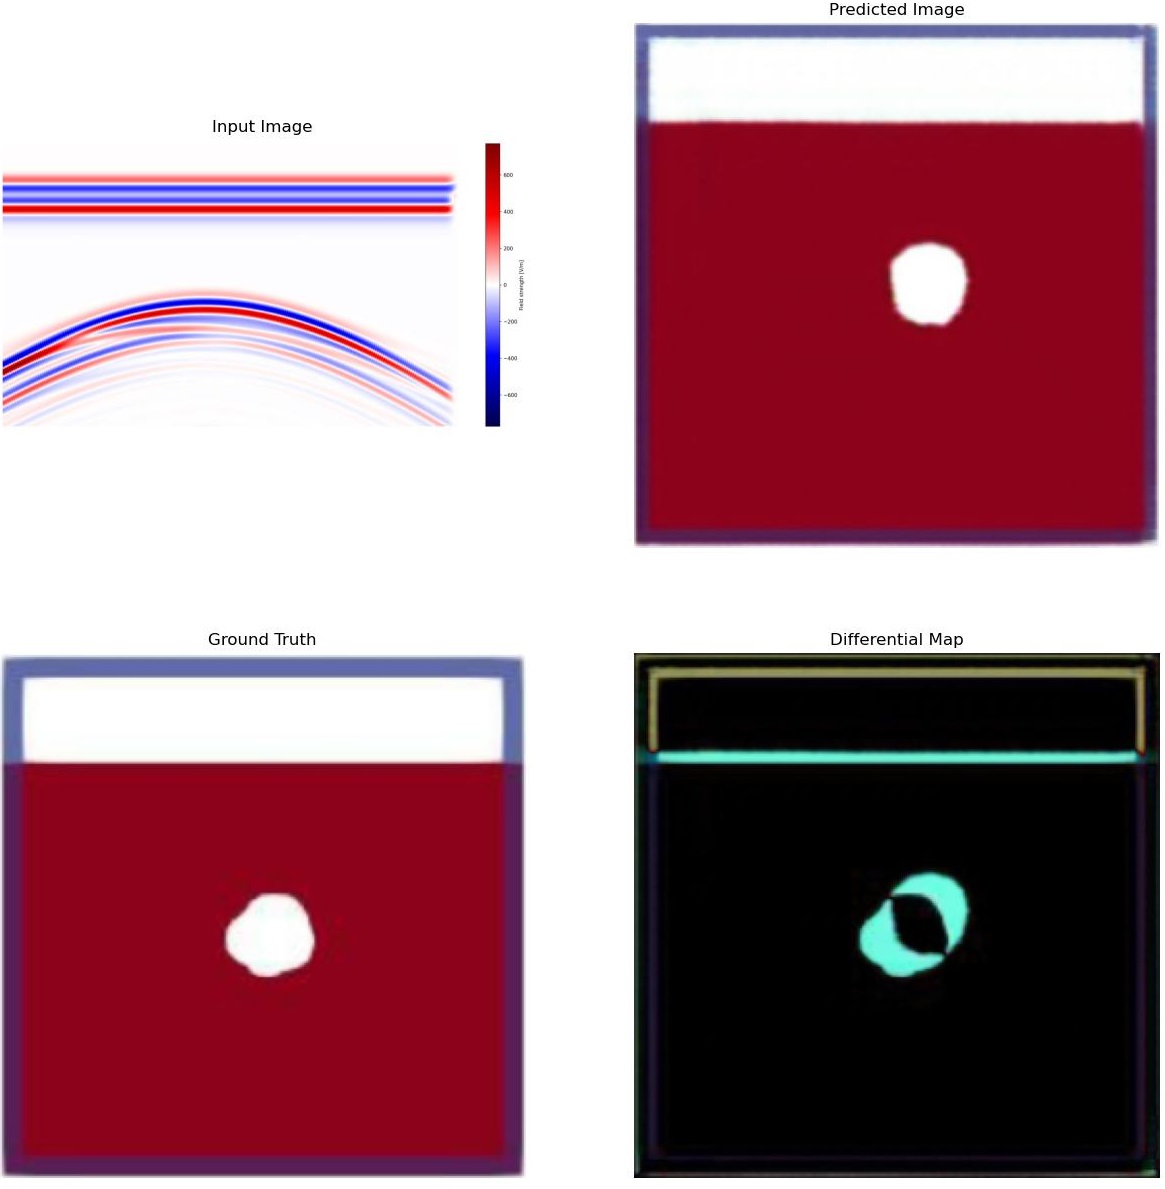
\includegraphics[scale=0.15]{gambar/diffMapSederhana.jpg}
  \caption{Visual Evaluation of Simple Shape Variation Data}
  \label{fig:diffmapsederhana}
\end{figure}

For data variations with simple objects, the first data will be taken because it has a matrix evaluation value that is closer to the average object shape variation from other data.
Visual evaluation of the data can be seen from Figure \ref{fig:diffmapsederhana}.
In the visual evaluation image, it can be seen that the intersection of the synthesis object and the original object is wide enough so that it has a fairly narrow error area.
This shows that the output model is able to show the position and size of the object, but still cannot show the shape of the object.

\begin{figure}[ht]
  \centering
  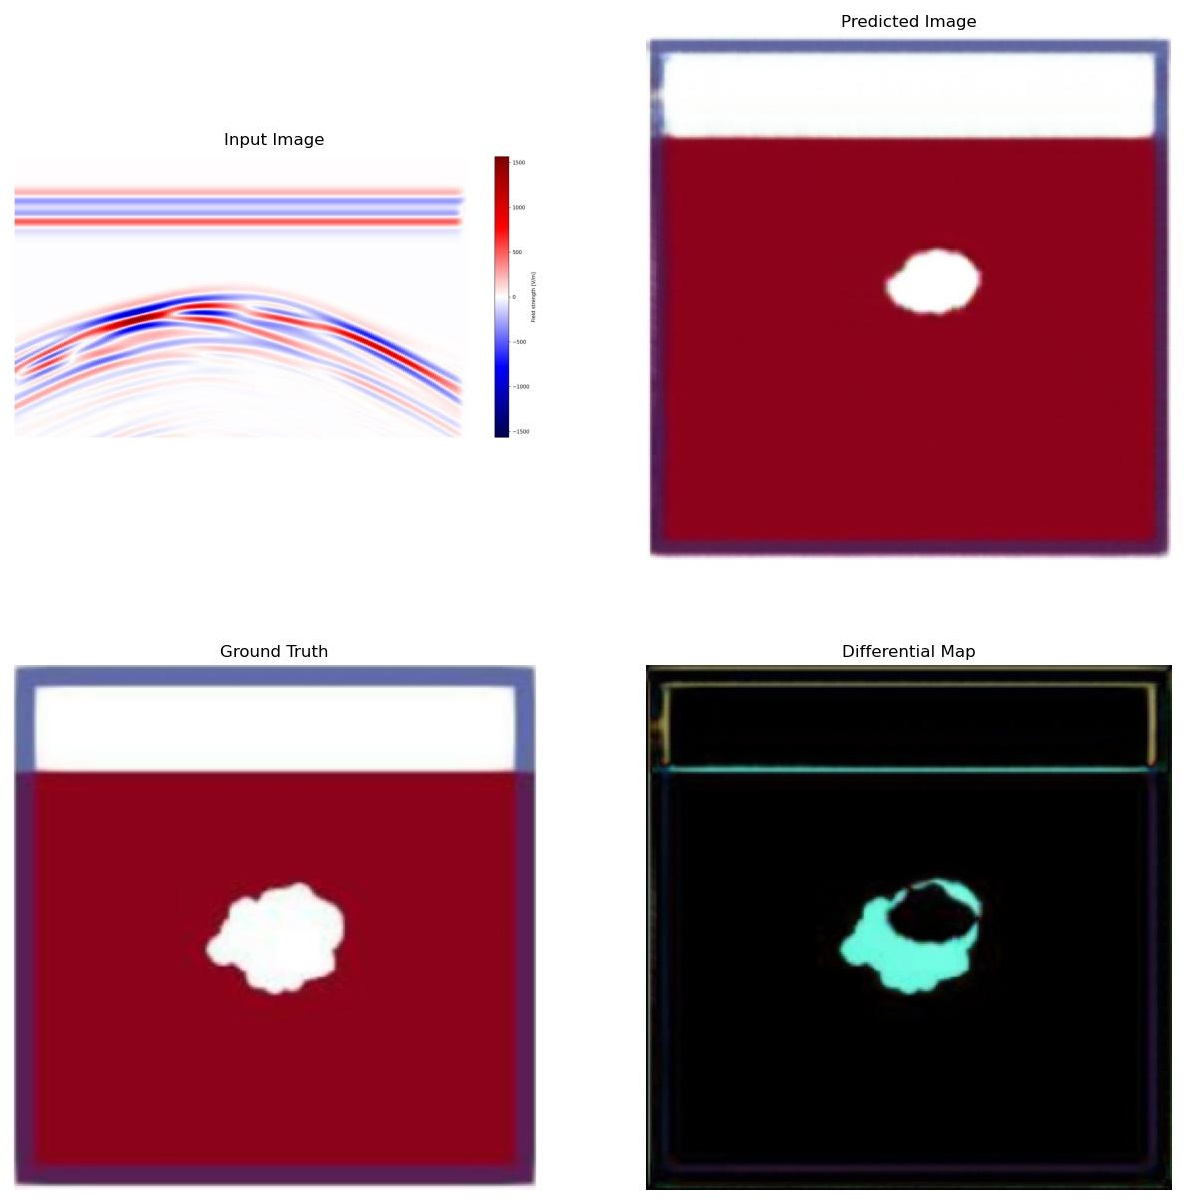
\includegraphics[scale=0.15]{gambar/diffMapKompleks.jpg}
  \caption{Evaluasi Visual Data Variasi Bentuk Kompleks}
  \label{fig:diffmapkompleks}
\end{figure}

For data variations with complex objects, the first data will be taken because it has a matrix evaluation value that is closer to the average object shape variation from other data.
Visual evaluation of the data can be seen from Figure \ref{fig:diffmapkompleks}.
In the visual evaluation image, it can be seen that the intersection of the synthesis image and the original image is almost a complete synthesis image.
This shows that the output model is able to show the position of the object, but still cannot show the shape and size of the object.

In the variation of object size, it can be seen that small-sized objects have a better average matrix evaluation value than large-sized objects.
The difference in the average matrix evaluation looks quite far between the two variations of the data.
The average RMS and MSE values of small data objects are smaller than the average RMS and MSE values of large data objects.
However, the SSIM data object's average value for small data objects is greater than the SSIM data object's average value for large data objects.

\begin{figure}[ht]
  \centering
  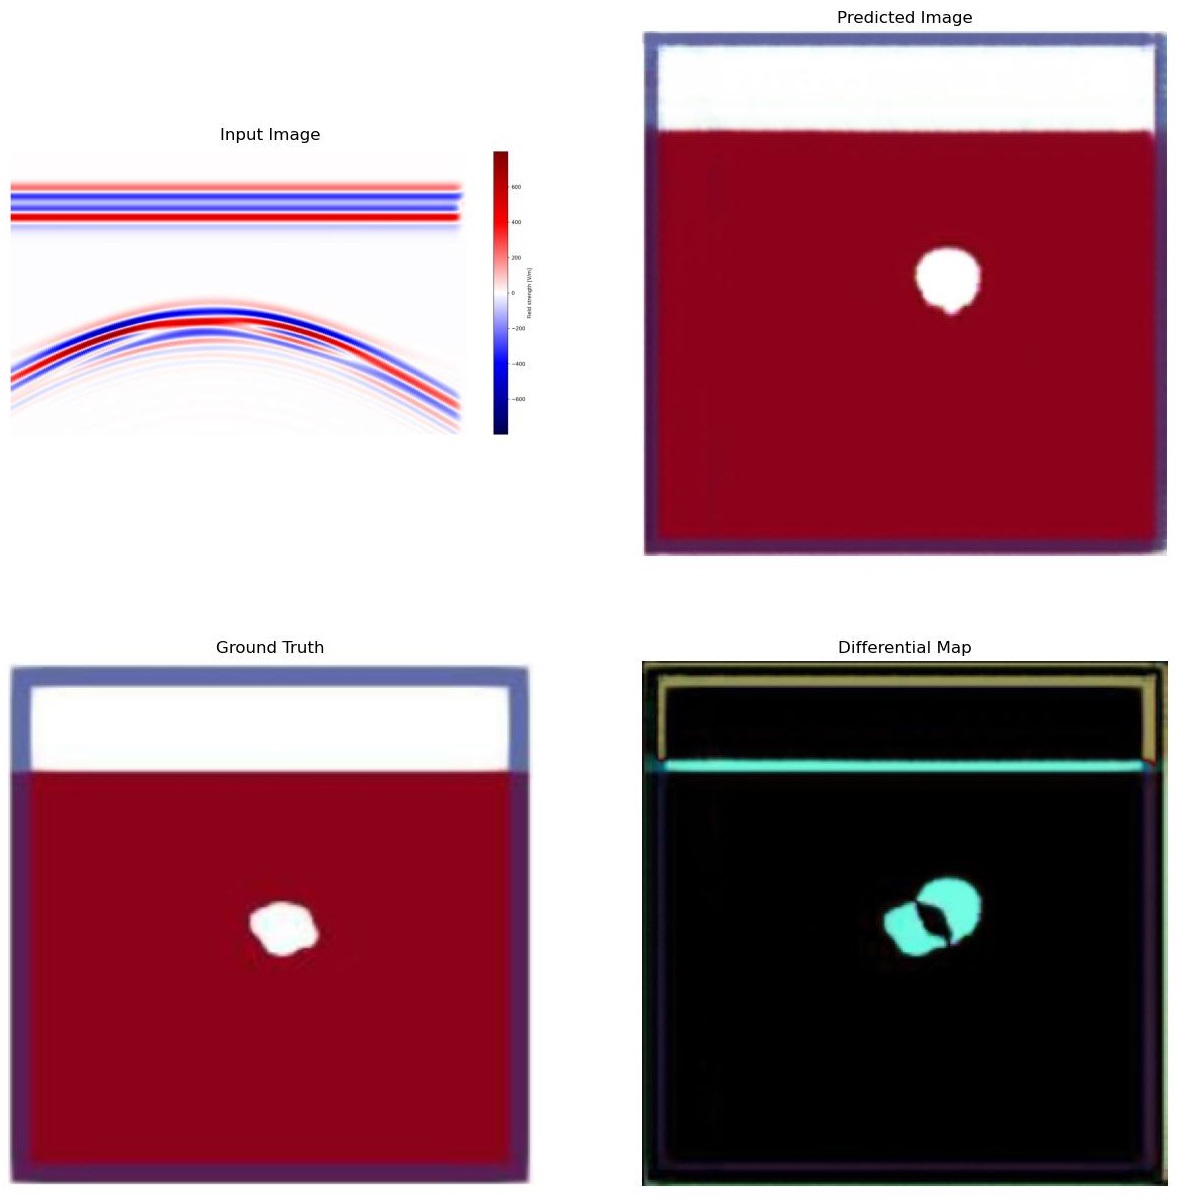
\includegraphics[scale=0.15]{gambar/diffMapKecil.jpg}
  \caption{Visual Evaluation of Small Size Variation Data}
  \label{fig:diffmapkecil}
\end{figure}

For data variations with small-sized objects, the fifth data will be taken because it has a matrix evaluation value that is closer to the average object size variation from other data.
Visual evaluation of the data can be seen from Figure \ref{fig:diffmapkecil}.
In the visual evaluation image, it can be seen that the intersection of the synthesis object and the original object is quite small so that it has a large enough error area.
This shows that the output model can almost show the position and size of the object, but still cannot show the shape of the object.

\begin{figure}[ht]
  \centering
  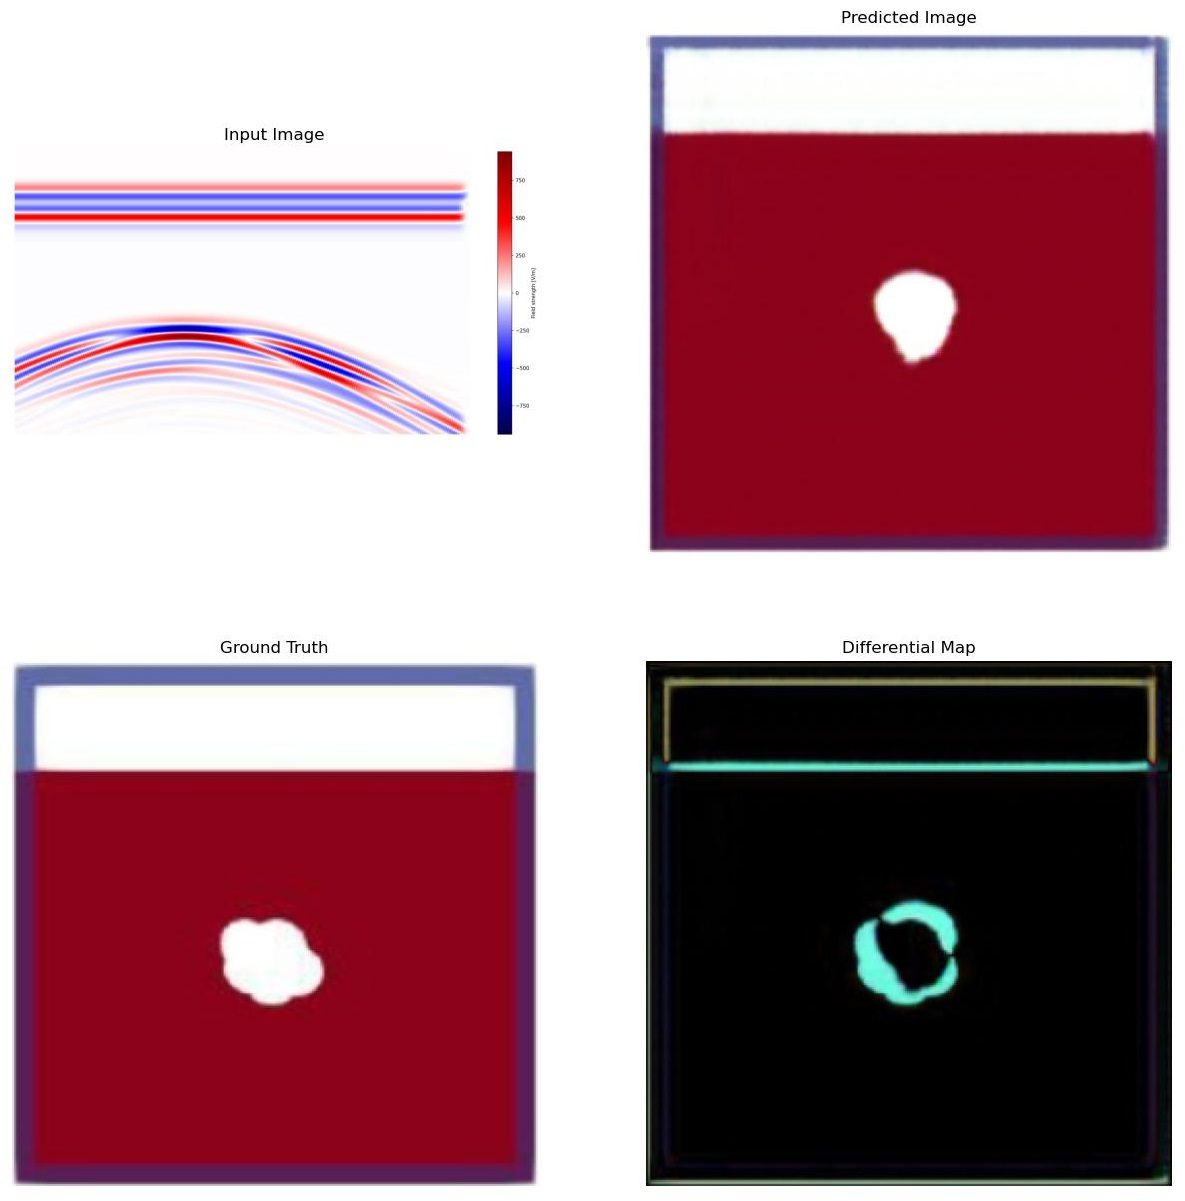
\includegraphics[scale=0.15]{gambar/diffMapBesar.jpg}
  \caption{Visual Evaluation of Large Size Variation Data}
  \label{fig:diffmapbesar}
\end{figure}

For data variations with large objects, the first data will be taken because it has a matrix evaluation value that is closer to the average object size variation from other data.
Visual evaluation of the data can be seen from Figure \ref{fig:diffmapbesar}.
In the visual evaluation image, it can be seen that the intersection of the synthesis object and the original object is narrow enough so that it has a large enough error area.
This shows that the model output can almost show the position of the object, but still cannot show the shape and size of the object.

In the variation of object position, it can be seen that objects with positions close to the surface have an average matrix evaluation value that is better than objects with positions far from the surface.
The difference in the average matrix evaluation looks quite far between the two variations of the data.
The average RMS and MSE values of object position data near the surface are smaller than the average RMS and MSE values of object position data far from the surface.
However, the SSIM average value of object position data near the surface is greater than the SSIM average value of object position data far from the surface.

\begin{figure}[ht]
  \centering
  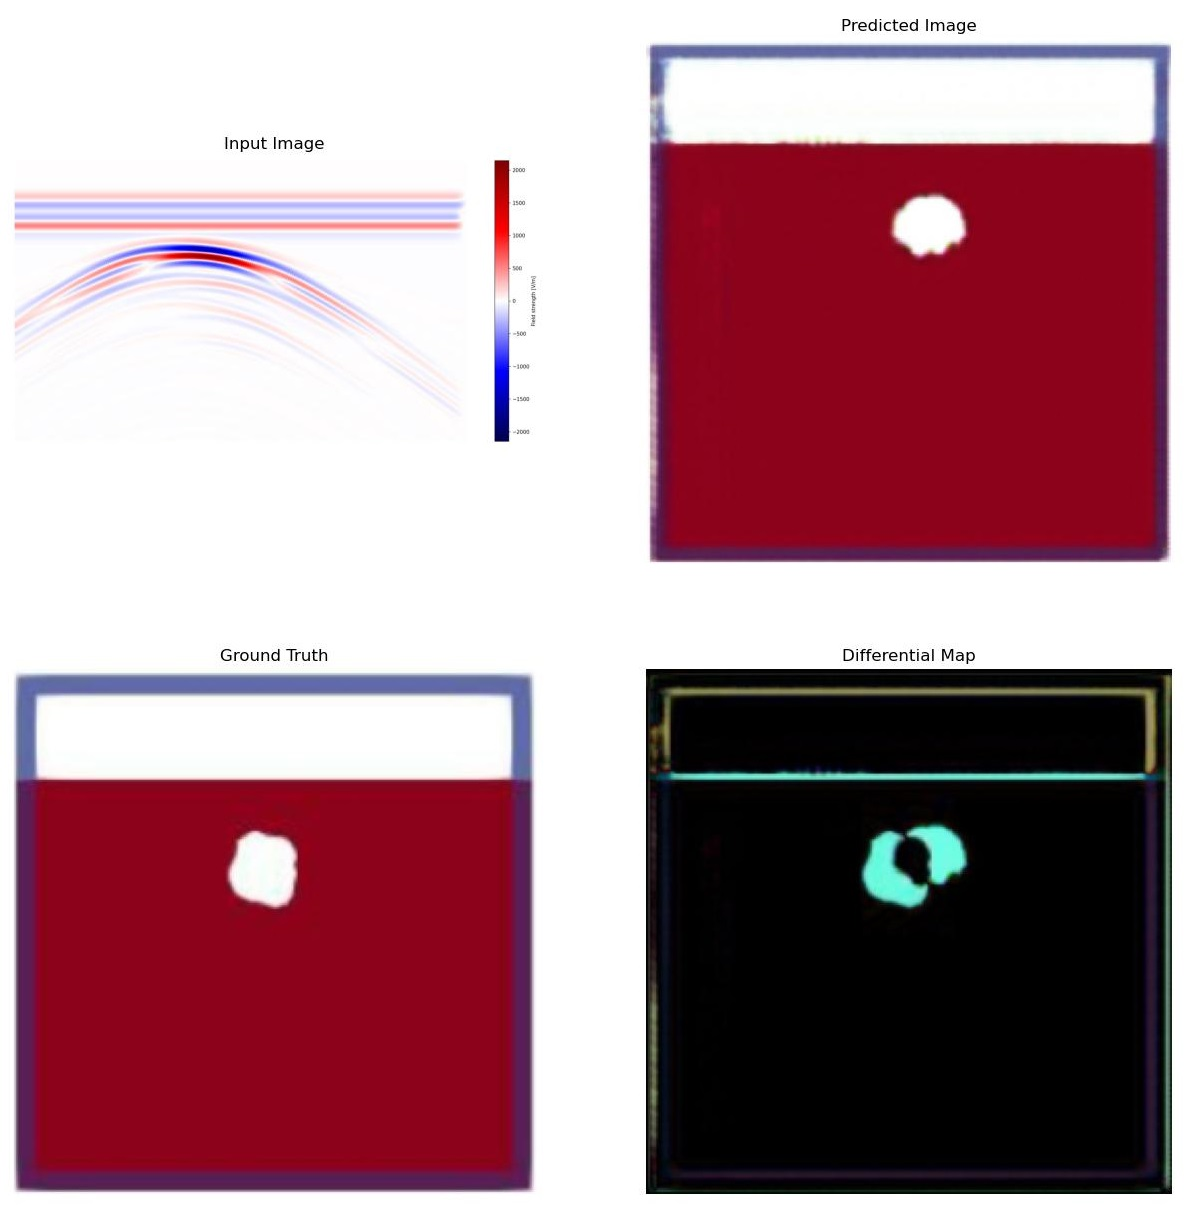
\includegraphics[scale=0.15]{gambar/diffMapDangkal.jpg}
  \caption{Visual Evaluation of Position Variation Data Close to Surface}
  \label{fig:diffmapdangkal}
\end{figure}

For data variations with object position close to the surface, the first data will be taken because it has a matrix evaluation value that is closer to the average object position variation from other data.
Visual evaluation of the data can be seen from Figure \ref{fig:diffmapdangkal}.
In the visual evaluation image, it can be seen that the intersection of the synthesis object and the original object is quite small so that it has a large enough error area.
This shows that the model output can almost show the position of the object, but still cannot show the shape and size of the object.

\begin{figure}[ht]
  \centering
  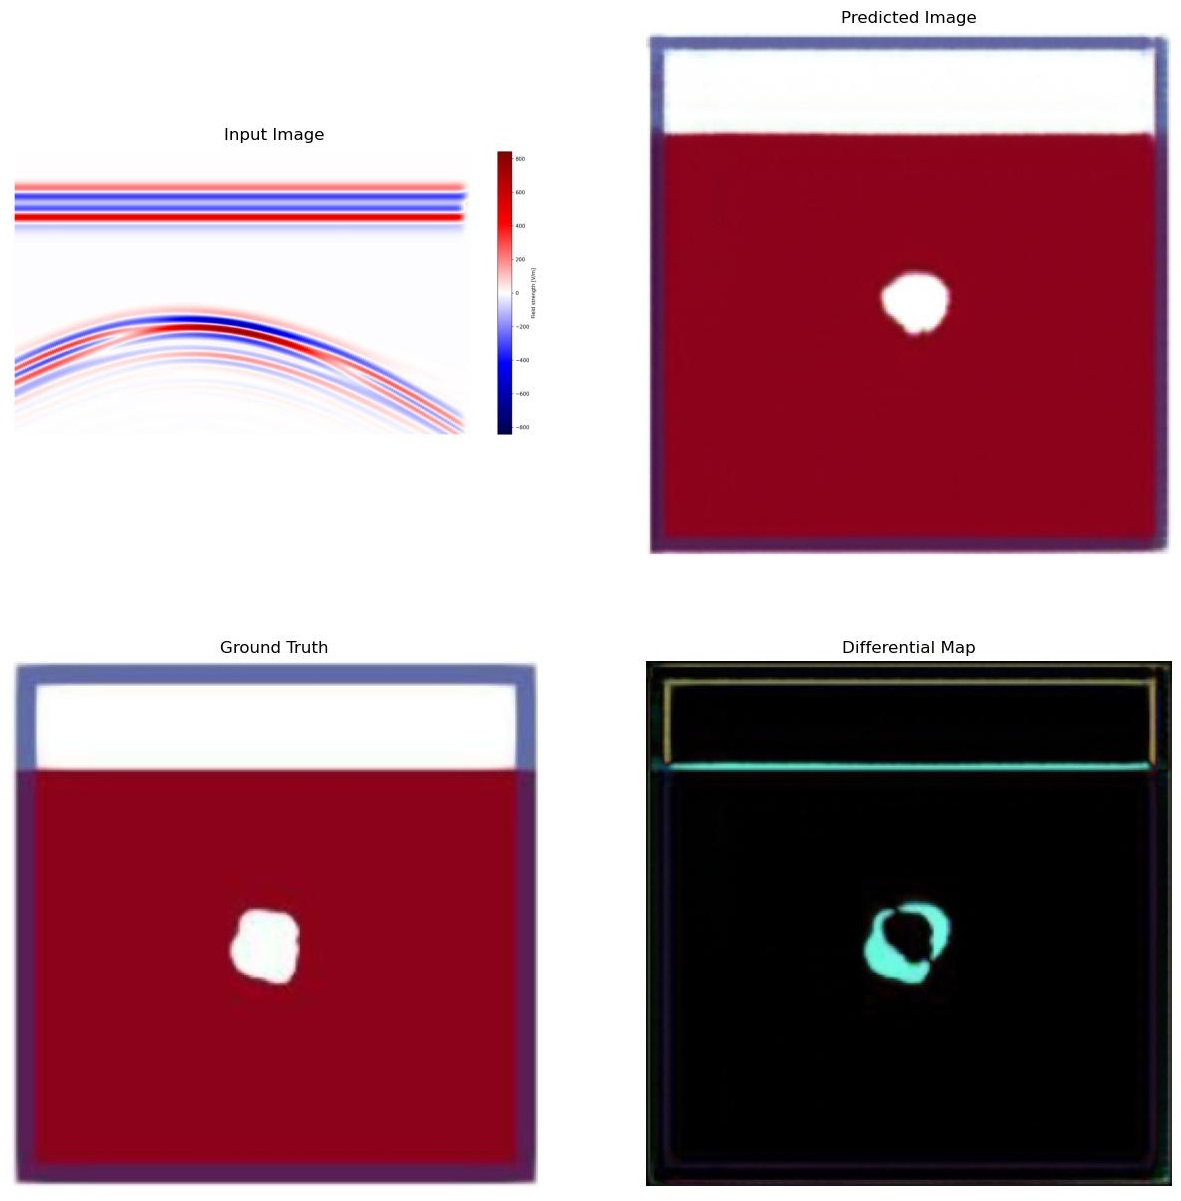
\includegraphics[scale=0.15]{gambar/diffMapDalam.jpg}
  \caption{Visual Evaluation of Distant Position Variation Data with Surface}
  \label{fig:diffmapdalam}
\end{figure}

For data variations with object positions far from the surface, a second data will be taken because it has a matrix evaluation value that is closer to the average object position variation from other data.
Visual evaluation of the data can be seen from Figure \ref{fig:diffmapdalam}
In the visual evaluation image, it can be seen that the intersection of the synthesis object and the original object is quite small so that it has a large enough error area.
This shows that the model output can almost show the position of the object, but still cannot show the shape and size of the object.

In the regular shape variations of objects, it can be seen that circle-shaped objects have an average matrix evaluation value that is worse than rectangular-shaped objects.
The difference in the average matrix evaluation looks quite far between the two variations of the data.
The average RMS and MSE values for circular object data are greater than the RMS and MSE average values for rectangular data objects.
However, the SSIM average value of circular data objects is greater than the average value of rectangular SSIM data objects.

\begin{figure}[ht]
  \centering
  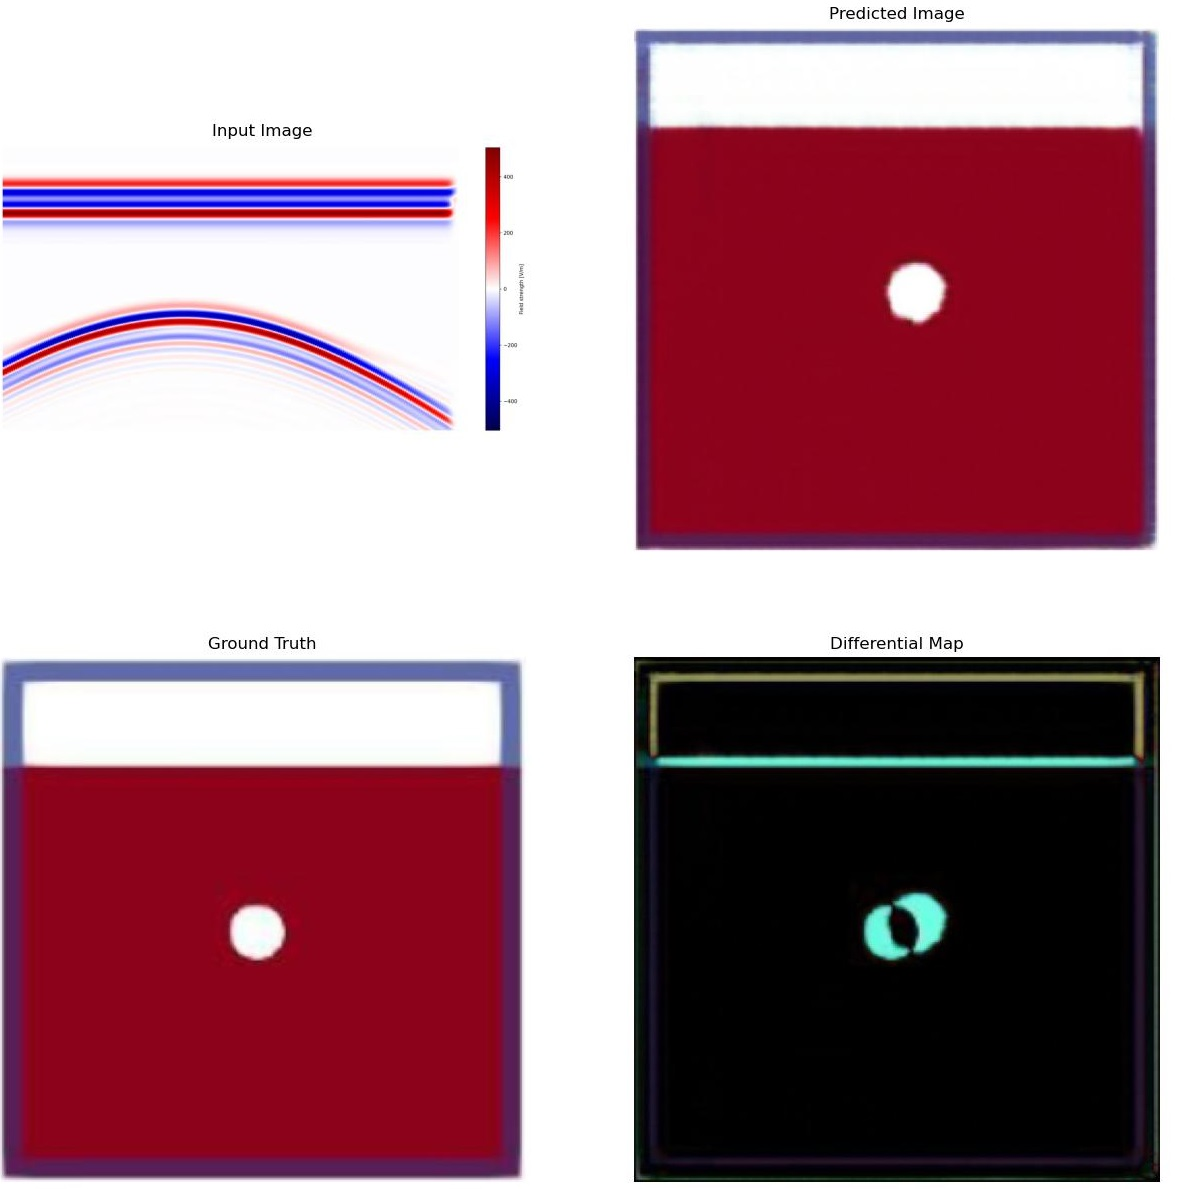
\includegraphics[scale=0.15]{gambar/diffMapLingkaran.jpg}
  \caption{Visual Evaluation of Regular Circle Shape Variation Data}
  \label{fig:diffmaplingkaran}
\end{figure}

For data variations with a circle shape, the fifth data will be taken because it has a matrix evaluation value that is closer to the average variation of the regular shape of objects from other data.
Visual evaluation of the data can be seen from Figure \ref{fig:diffmaplingkaran}.
In the visual evaluation image, it can be seen that the intersection of the synthesis object and the original object is quite small so that it has a large enough error area.
This shows that the model output can almost show the position of the object, but still cannot show the shape and size of the object.

\begin{figure}[ht]
  \centering
  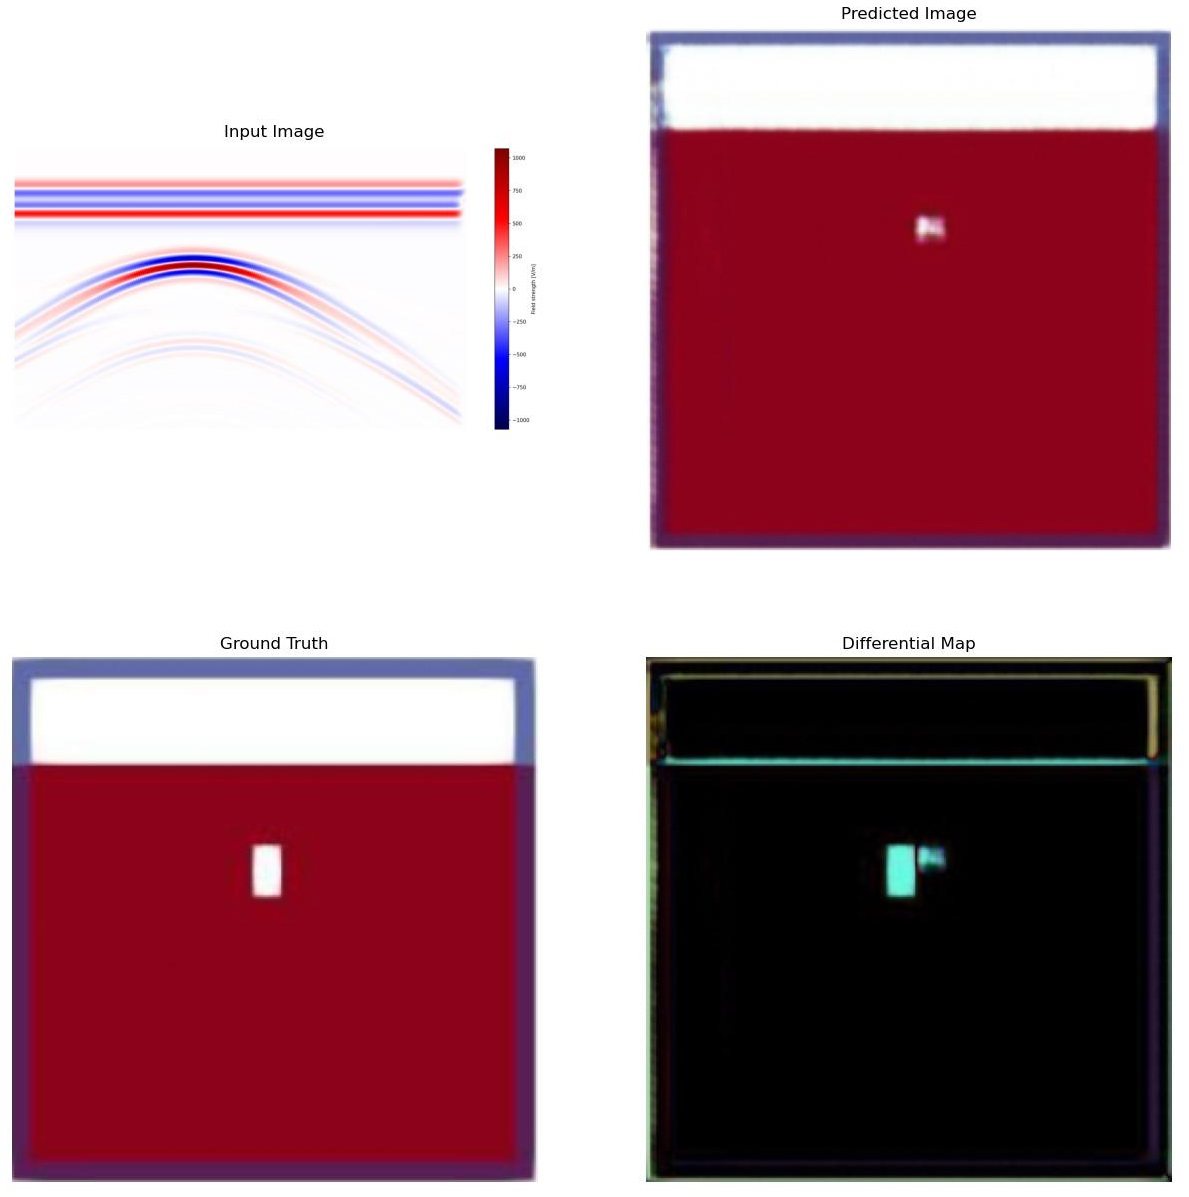
\includegraphics[scale=0.15]{gambar/diffMapSegi4.jpg}
  \caption{Visual Evaluation of Quadrilateral Regular Shape Variation Data}
  \label{fig:diffmapsegi4}
\end{figure}

For data variations with a rectangular shape, the first data will be taken because it has a matrix evaluation value that is closer to the average variation of the regular shape of objects from other data.
Visual evaluation of the data can be seen from Figure \ref{fig:diffmapsegi4}.
In the visual evaluation image, it can be seen that the intersection of the synthesis object and the original object is quite small so that it has a large enough error area.
This shows that the model output can almost show the position of the object, but still cannot show the shape and size of the object.

\section{Conclusions and recommendations}
 
The results of the research using the GAN model to reconstruct GPR B-scan signals on irregularly shaped objects show that during the training process of the GAN model, the Total Generator Loss graph experiences a decrease in value from start to finish, while the Total Discriminator Loss graph experiences a decrease in value at the beginning, then an increase in value at the end.
This shows that the Generator is getting better at producing the desired image. However, the Discriminator initially gets better at distinguishing real data from fake data, but at the end of the training it becomes increasingly difficult to distinguish between them.
Based on the matrix evaluation results of 40 GPR test data ($RMS_{average}$ = 0.247, $MSE_{average}$ = 0.070, $SSIM_{average}$=0.833), the GAN model works better in synthesizing images of subsurface structures for objects with positions close to the surface (RMS = 0.239, MSE = 0.63, SSIM = 0.841), circular (RMS = 0.2 37, MSE = 0.064, SSIM = 0.843) and rectangular (RMS = 0.219, MSE = 0.058, SSIM = 0.838).
However, based on the results of the visual evaluation, the output model is quite capable of showing the position of the object, and still cannot show the shape and size of the object for each variation.
The GAN model is able to reconstruct irregular objects buried in concrete based on GPR B-scan signals more quickly with an average inference time of 0.423 seconds

For further development in this final project research, the authors suggest to be able to reproduce the train data for variations in the shape and size of objects in order to maximize the results of image predictions.
New types of objects and propagation media for GPR signals simulated by gprMax can also be added.
Further research can also be developed for other forms of GPR signals, namely A-scan and C-scan.

\section{Attachment}

All purposes used in making this research are stored on GitHub which can be accessed via the link : MehhTerserah/TA-072-19-0040 (github.com)

\section{Expression of Thanking}

The author J.P.S would like to thank the author's family who helped the author spiritually and materially in the preparation of this article,
Mr. Dr. Supeno Mardi Susiki Nugroho, ST., MT. as Head of Computer Engineering Department, Faculty of Intelligent Electrical and Informatics Technology (ELECTICS), Sepuluh Nopember Institute of Technology (ITS),
Mr. Dion Hayu Fandiantoro, S.T., M.Eng. as Advisor I and Mr. Arief Kurniawan, S.T, M.T. as Co-Advisor II who always gives directions while working on this final project research,
and The entire ITS Computer Engineering extended family, especially the 2019 generation students, who have provided a lot of assistance to the writer.

\begin{thebibliography}{00}
\bibitem{a1} Neal, A. (2004). Ground-penetrating radar and its use in sedimentology: Principles, problems and progress. Earth-Science Reviews, 66(3), 261–330. https://doi.org/https://doi.org/10.1016/j.earscirev.2004.01.004
\bibitem{a2} PUPR, B. (2015). Diklat pemeliharaan jembatan ii : Modul 2 perbaikan kerusakan berdasarkan bahan. https:/ /simantu.pu.go.id/epel/edok/2d370 Modul 2 - Perbaikan Kerusakan Berdasarkan Bahan.pdf
\bibitem{a3} Gurel, L., and Oguz, U. (2000). Three-dimensional fdtd modeling of a ground-penetrating radar. IEEE Transactions on Geoscience and Remote Sensing, 38(4), 1513–1521. https://doi.org/10.1109/36.851951
\bibitem{a4} van den Bosch, I., Lambot, S., Huynen, I., Marc, A., and Druyts, P. (2006). Accurate and efficient modeling of monostatic gpr signal of dielectric targets buried in stratified media. Journal of Electromagnetic Waves and Applications, 20, 283–290. https://doi.org/10.1163/156939306775701704
\bibitem{a5} Liu, H., Xing, B., Wang, H., Cui, J., and Spencer, B. F. (2019). Simulation of ground penetrating radar on dispersive media by a finite element time domain algorithm. Journal of Applied Geophysics, 170, 103821. https: / / doi.org/ https: / / doi.org/10.1016/ j.jappgeo.2019.103821
\bibitem{a6} Irving, J., Knoll, M., and Knight, R. (2007). Improving crosshole radar velocity tomograms: A new approach to incorporating high-angle traveltime data. Geophysics, 72, J31–J41. https://doi.org/10.1190/1.2742813
\bibitem{a7} Liu, S., Lei, L., Fu, L., and Wu, J. (2014). Application of pre-stack reverse time migration based on fwi velocity estimation to ground penetrating radar data. Journal of Applied Geophysics, 1–7.
\bibitem{a8} Kruk, J., Liu, T., Mozaffari, A., Gueting, N., Klotzsche, A., Vereecken, H., Warren, C., and Giannopoulos, A. (2018). Gpr full-waveform inversion, recent developments, and future opportunities, 1–6. https://doi.org/10.1109/ICGPR.2018.8441667
\bibitem{a9} Ishitsuka, K., Iso, S., Onishi, K., and Matsuoka, T. (2018). Object detection in ground-penetrating radar images using a deep convolutional neural network and image set preparation by migration. International Journal of Geophysics, 2018, 1–8. https:/ /doi.org/10.1155/2018/9365184
\bibitem{a10} Ren, S., He, K., Girshick, R., and Sun, J. (2017). Faster r-cnn: Towards real-time object detection with region proposal networks. IEEE Transactions on Pattern Analysis and Machine Intelligence, 39(6), 1137–1149. https://doi.org/10.1109/TPAMI.2016.2577031
\bibitem{a11} Jiang, P., Gu, F., Tu, C., and Chen, B. (2018, May). Difnet: Semantic segmentation by diffusionnetworks.
\bibitem{a12} Goodfellow, I., Pouget-Abadie, J., Mirza, M., Xu, B.,Warde-Farley, D., Ozair, S., Courville, A., and Bengio, Y. (2014). Generative adversarial networks. Advances in Neural Information Processing Systems, 3. https://doi.org/10.1145/3422622
\bibitem{a13} Liu, B., Ren, Y., Liu, H., Xu, H., Wang, Z., Cohn, A., and Jiang, P. (2021). Gprinvnet: Deep learning-based ground-penetrating radar data inversion for tunnel linings. IEEE Transactions on Geoscience and Remote Sensing, PP, 1–21. https://doi.org/10.1109/TGRS. 2020.3046454
\bibitem{b1} Rice,W. B. D. (2019). Applying generative adversarial networks to intelligent subsurface imaging and identification. ArXiv, abs/1905.13321
\bibitem{b2} Shen, Z., Erdogmus, E., Morcous, G., Cheng, C., Shang, Z., McCabe, T., and Kodsy, A. (2020). Early detection of near-surface void defects in concrete pavement using drone based thermography and gpr methods.
\bibitem{b3} Isola, P., Zhu, J.-Y., Zhou, T., and Efros, A. (2017). Image-to-image translation with conditional adversarial networks, 5967–5976. https://doi.org/10.1109/CVPR.2017.632
\bibitem{c1} Ronneberger, O., Fischer, P., and Brox, T. (2015). U-net: Convolutional networks for biomedical image segmentation. LNCS, 9351, 234–241. https://doi.org/10.1007/978-3-319-24574-4 28
\end{thebibliography}

\end{document}
